\documentclass[12pt]{article}
\usepackage[a4paper, width=6.3in, left=1.3in, right=1.3in, height=9.2in, top=1.1in]{geometry}
\usepackage[T1]{fontenc}
\usepackage[utf8]{inputenc}
\usepackage{lmodern}
\usepackage{amsfonts,amsmath,amssymb,amsthm}
\usepackage[htt]{hyphenat}
\usepackage{fancyhdr}
\usepackage[nottoc,notlot,notlof]{tocbibind}
\usepackage{verbatim}
\usepackage{graphicx}
\usepackage{wrapfig}
\usepackage{caption}
\usepackage[table]{xcolor}
\fancyfoot[R]{\thepage}
\usepackage{ctable}
\usepackage{color} %red, green, blue, yellow, cyan, magenta, black, white
\usepackage[title, titletoc]{appendix}
\usepackage{array}
\usepackage{hyperref}
\usepackage{listings}
\usepackage[noabbrev]{cleveref}
\usepackage{subfig}

\renewcommand{\thesubfigure}{Figure \arabic{subfigure}}
\captionsetup[subfigure]{labelformat=simple, labelsep=colon}

\newcolumntype{C}[1]{>{\centering\arraybackslash}p{#1}}

\definecolor{mygreen}{RGB}{28,172,0} % color values Red, Green, Blue
\definecolor{mydarkgreen}{RGB}{28,132,0} 
\definecolor{mylilas}{RGB}{170,55,241}
\definecolor{mygrey}{RGB}{123,123,123}
\definecolor{myorange}{RGB}{230,80,80}
\definecolor{codebackground}{RGB}{230,230,230}
\definecolor{mydarkblue}{RGB}{0,102,153}


\newcommand{\mbeq}{\overset{!}{=}}

% Paths to java files. Note these might give errors when working on a different computer
\newcommand{\finmathlib}{C:/Users/marku/IdeaProjects/finmath-lib/src/main/java/net/finmath}
\newcommand{\libMC}{\finmathlib/montecarlo}
\newcommand{\codepath}{C:/Users/marku/IdeaProjects/master-thesis-default-forward-rate-models/src}
\newcommand{\codepathmodels}{\codepath/main/java/info/quantlab/masterthesis}
\newcommand{\codedlmm}[1]{\codepathmodels/defaultablelibormodels/#1}
\newcommand{\codecovdlmm}[1]{\codepathmodels/defaultablecovariancemodels/#1}
\newcommand{\codeprocess}[1]{\codepathmodels/process/#1}

\newcommand{\fig}[1]{figures/#1}

\newcommand{\einsch}{\,\rule[-5pt]{0.4pt}{15pt}\,{}}
%\newcommand{\EQB}[1]{\mathbb{E}^{\mathbb{Q}^B}\left[#1\right]}
\parindent 0ex
\renewcommand{\baselinestretch}{1.5}
\newtheorem{assumption}{Assumption}[section]
\newtheorem{theorem}{Theorem}[section]
\newtheorem{lemma}[theorem]{Lemma}
\newtheorem{notation}[theorem]{Notation}
\newtheorem{remark}[theorem]{Remark}
\newtheorem{definition}[theorem]{Definition}

\crefname{assumption}{assumption}{assumptions}
\crefname{notation}{notation}{notations}
\crefname{remark}{remark}{remarks}


\renewcommand{\labelenumi}{\em{(\roman{enumi})}}
\renewcommand{\labelenumii}{\em{(\alph{enumii})}}
\captionsetup[figure]{skip=0pt}


\lstset{
	inputencoding		=utf8,
	postbreak			=\raisebox{0ex}[0ex][0ex]{\ensuremath{\color{red}\hookrightarrow\space}},
	language			=Java,
	basicstyle			=\ttfamily\scriptsize,
	backgroundcolor		=\color{codebackground},
	tabsize				=3,
	captionpos			=b,
	morekeywords		={java2tikz},
	keywordstyle		=\color{orange},
	morekeywords		=[2]{1},
	keywordstyle		=[2]{\color{black}},
	identifierstyle		=\color{black},
	stringstyle			=\color{mygreen},
	commentstyle		=\color{mydarkgreen},
	showstringspaces	=false,
	showspaces			=false,
	numbers				=left,
	numberstyle			=\tiny\color{black},
	numbersep			=5pt,
	breaklines,
	breakatwhitespace,
	emph=[1]{RandomVariable,ProcessModel,MonteCarloProcess,LIBORMarketModel,DefaultableLIBORMarketModel,SimulationModel,CalculationException},emphstyle=[1]\color{mydarkblue}, %some words to emphasise
	emph=[2]{SPREADS}, emphstyle=[2]\color{mylilas},    
}


\begin{document}
	\begin{titlepage}
		
		
		
		\begin{center}
			\normalsize{Ludwig-Maximilians-Universität München \\
				Mathematisches Institut}\\[15ex]
			
			\LARGE{Master's Thesis}\\[1.2ex]	
			\LARGE{\textbf{Default Forward Rate Models for the Valuation of Loans including Behavioral Aspects}} \\[2.5ex]
			\Large{\textit{Markus Parhofer}}\\[9ex]
		\end{center}
		
		
		\begin{center}
			\includegraphics[width=1.8in]{\fig{siegel}}\\[13ex]
		\end{center}
		
		\begin{center}
			\normalsize{}
			Under supervision of\\
			Prof. Dr. Christian Fries\\
			\today\
			\\
		\end{center}
		
	
	
	
\end{titlepage}

	% ------------------------------Content------------------------
\tableofcontents
\thispagestyle{empty}
\clearpage


	
	
	
	% ----------- Intro -----------
	
	
	
	\section{Introduction}
	\color{red}The valuation of loans in financial markets is crucial for creditors and debtors alike. Understanding and measuring the risks associated with interest rates, especially default risk, is essential for valuing and collateralizing financial products\color{black}. This master's thesis focuses on extending the existing and well researched discrete forward rate models (short: LIBOR models) to account for default risk, building upon the work of Professor Dr. Christian Fries.
	
	
	\subsection{Motivation}
	While they are very popular for the valuation of interest rate products, traditional LIBOR models do not account for the risk of default, which is a crucial aspect in financial mathematics. 
	
	Using exogenous models to adjust for the probability of default (PD) and a loss given default (LGD) is a work around, that is widely used in praxis. However, there is another solution that directly links the interest rate model with the risk of default.\\
	Prof. Fries' Paper on "Discrete Forward Rate Model with	Covariance Structure guaranteeing Positive Credit Spreads" \cite{friesDLMM} provides a foundation for models that address this gap by incorporating default risk dynamics directly into the LIBOR model.\\
	This begs the question of how to apply these models to pricing and how this impacts prices which are otherwise only driven by interest rates.
	
	\subsection{Aim of the thesis}
	
	This thesis aims to contribute to the field by describing the discrete forward rate models, developing a valuation methodology with this framework and providing an implementation in the programming language Java for evaluating its usability.\\
	
	We begin by stating some fundamentals in section \ref{sec:Fundamentals}, which are mainly results from financial mathematics in continuous time.\\
	In section \ref{sec::LIBORModel} we describe the traditional LIBOR market model, which is given by a set of stochastic differential equations.\\
	Throughout section \ref{sec:defaultableLMM} we describe the model developed by Prof. Fries and derive some implications.\\
	We then develop a general pricing methodology in section \ref{sec:pricing} and derive valuation formulas for some specific products.\\
	Section \ref{sec:numerical} gives an overview of the actual numerical specification of the model and also displays results gained from the usage.\\
	Finally, in section \ref{sec:conclusion} we conclude the thesis by summarizing key findings, outlining limitations, and offering recommendations for future research.
	
	
	\subsection{Preliminaries}
	The thesis is aimed at an audience that has a deep analytical background and a basic knowledge in probability theory and financial mathematics.\\
	A list of required topics may include, but is not limited to
	\begin{itemize}
		\item Brownian Motions and martingales,
		\item stochastic integration,
		\item Itô stochastic processes and
		\item definition of and theorems on arbitrage free markets.
	\end{itemize}
	Furthermore we assume a fundamental understanding of what these mathematical concepts imply on the real world and the other way around: How are the mathematical concepts motivated by the economical world?
	
	
	
	
	% --------------------------- Fundamentals----------------------
	
	
	
	\pagebreak
	\section{Fundamentals}\label{sec:Fundamentals}
	In this section we provide some fundamentals for the thesis. Many of the results mentioned here can also be found in different versions in other scientific papers. We will generally stick to the lecture notes of the course "Stochastic Calculus and Arbitrage Theory in Continuous Time" by Professor Meyer-Brandis at the Ludwig-Maximilians-University in Munich \cite{fima2Lecture}.
	
	\subsection{Probability Theory}
	In our whole thesis we assume a filtered probability space
	\begin{align*}
		(\Omega, \mathcal{G}, \mathbb{G}, \mathbb{Q})
	\end{align*}
	where
	\begin{itemize}
		\item $\Omega$ is the set of all states,
		\item $\mathcal{G}$ is a $\sigma$-algebra,
		\item $\mathbb{G} = (\mathcal{G}_t)_{t \in \left[0,\tilde{T}\right]}$ is a filtration with $\mathcal{G}_t \subset \mathcal{G} \quad \forall t \in [0,\tilde{T}]$, $\mathcal{G}_0 = \{\Omega, \emptyset \}$ and
		\item $\mathbb{Q}$ is a probability measure on $\mathcal{G}$.
	\end{itemize}
	$\mathbb{G}$ is the pricing filtration, which captures all states of all traded assets at each time $t$. Hence we implicitly assume all market values that we encounter to be $\mathbb{G}$-adapted.\\
	Let us cover some further notations.
	\begin{notation}
		Let $X=(X_t)_{t\in \left[0,\tilde{T}\right]}$ and $Y=(Y_t)_{t\in \left[0,\tilde{T}\right]}$ be Itô stochatic processes and $W$ be a Brownian Motion with:
		\begin{align*}
			X_t &= X_0 + \int_{0}^{t}\mu^X_s ds + \int_{0}^{t}\phi_s dW_s, \\
			Y_t &= Y_0 + \int_{0}^{t}\mu^Y_s ds + \int_{0}^{t}\psi_s dW_s.
		\end{align*}
		The \emph{sharp bracket} or \emph{quadratic variation} of $X$ is 
		\begin{align*}
			\left\langle X \right\rangle_t = \int_{0}^{t}\phi_s^2 ds.
		\end{align*}
		The \emph{quadratic covariation} of $X$ and $Y$ is 
		\begin{align*}
			\left\langle X, Y \right\rangle_t = \int_{0}^{t}\phi_s \psi_s ds.
		\end{align*}
		For a $n$-dimensional Brownian Motion $W = (W^i)_{i\in\{1,...,n\}}$ and therefore $n$-dimensional diffusion processes $\phi=(\phi^i)_{i \in \{1,..., n\}}$, $\psi=(\psi^i)_{i \in \{1,..., n\}}$ the quadratic covariation is
		\begin{align*}
			\left\langle X, Y \right\rangle_t = \sum_{i=1}^{n} \int_{0}^{t} \phi^i_s \psi^i_s ds
		\end{align*}
	\end{notation}
	For convenience we state a formula for stochastic integration by parts and an extended version of Itô's theorem:
	\begin{lemma}
		Let $X$ and $Y$ be two Itô stochastic processes. Then
		\begin{align*}
			X_t Y_t = X_0 Y_0 + \int_{0}^{t}X_sdY_s + \int_{0}^{t}Y_sdX_s + \left\langle X, Y\right\rangle_t \quad \text{for }t \in \left[0,\tilde{T}\right]
		\end{align*}
	\end{lemma}
	\begin{proof}
		See \cite{fima2Lecture}, page 51. %TODO: Add line where this is done.
	\end{proof}
	\begin{theorem}
		Let $X$ be an Itô stochastic process, $f: \mathbb{R}^n \times [0,\tilde{T}] \rightarrow \mathbb{R}, \; (x,t) \rightarrowtail f(x, t)$ be two times differentiable in $x$ and differentiable in $t$. Then
		\begin{align*}
			f(X_t, t) = \;&f(X_0, 0) + \int_{0}^{t}(\partial_{t}f)(X_s, s)ds + \sum_{i=1}^{n}\int_{0}^{t}(\partial_{x^i}f)(X_s, s)dX^i_s \\
			&+ \frac{1}{2} \sum_{i,j=1}^{n}\int_{0}^{t}(\partial^2_{x^ix^j}f)(X_s, s)d\left\langle X^i, X^j\right\rangle_s
		\end{align*}
		
	\end{theorem}
	\begin{proof}
		See \cite{fima2Lecture}, page 52. %TODO: Add line where this is done.
	\end{proof}
	
	Through Itô's formula we can prove the following statement.
	\begin{lemma}\label{lm:logNormalDyn}
		Let $W=(W^i)_{i\in \{1, ..., d\}}$ be a d-dimensional Brownian Motion, $\mu$ be a 1-dimensional and $\sigma = (\sigma^i)_{i\in \{1, ..., d\}}$ a $d$-dimensional stochastic process. Let following stochastic differential equation (SDE) be given:
		\begin{align}\label{eq:lognormalSDE}
			\begin{aligned}
				dY_t &= Y_t \mu_t dt + Y_t \sigma_t \cdot dW_t,\\
				Y_0 &= y,
			\end{aligned}
		\end{align}
		where $y > 0$.\\
		Then the solution of \cref{eq:lognormalSDE} is \begin{align}\label{eq:lognormalSDENormalized}
			\begin{aligned}
				Y_t &= \exp(X_t),\\
				X_t &= X_0 + \int_{0}^{t}\mu_s - \frac{1}{2}\sum_{i=1}^{d}(\sigma^i_s)^2ds + \int_{0}^{t}\sigma_s \cdot dW_s,\\
				X_0 &= \log(y).
			\end{aligned}
		\end{align}
	\end{lemma}
	\begin{proof}
		We use Itô's formula on \cref{eq:lognormalSDENormalized} with $f(x) = \exp(x)$, hence 
		\begin{align*}
			(\partial_xf)(x) = \exp(x), \quad (\partial^2_{xx})(x) = \exp(x).
		\end{align*}
		We get (in SDE format):
		\begin{align*}
			dY_t &= d\exp(X_t) = \exp(X_t)dX_t + \frac{1}{2}\exp(X_t)d\left\langle X \right\rangle_t\\
			&=	Y_t\left(\left(\mu_t -\frac{1}{2}\sum_{i=1}^{d}(\sigma^i_t)^2\right)dt + \sigma_t \cdot dW_t\right) + \frac{1}{2}Y_t \sum_{i=1}^{d}(\sigma^i_t)^2 dt\\
			&= Y_t \mu_t dt + Y_t \sigma_t \cdot dW_t,
		\end{align*}
		which yields \cref{eq:lognormalSDE}.
	\end{proof}
	\begin{remark}
		It is easy to see that because of the relation 
		\begin{align*}
			Y_t = \exp(X_t),
		\end{align*}
		it holds that $Y_t > 0$ for all $t \in [0,\tilde{T}]$.
	\end{remark}
	
	\subsection{Financial Mathematics}
	While the reader should have a deep understanding of what arbitrage is and how to avoid it when pricing financial products, we formulate the following two fundamental results as a reminder.
	\begin{theorem}
		Following statements are equivalent:
		\begin{itemize}
			\item The market is arbitrage-free and complete.
			\item There exists exactly one probability measure $\mathbb{Q}^B$ w.r.t. a numeraire $B$, such that the price process of every traded asset discounted by the numeraire $\frac{X}{B}$ is a martingale w.r.t. the filtration $\mathbb{G}$.
		\end{itemize}
	\end{theorem}
	\begin{proof}
		See \cite{fima2Lecture}, page 92 and 93. %TODO: Add line where this is done.
	\end{proof}
	This directly gives us a notation for the price of any product in an arbitrage-free and complete market.
	\begin{lemma}
		Let $X$ be the payoff of a $T$-claim. Then the arbitrage-free price of the claim at any time $t\in \left[0, T\right]$ is
		\begin{align*}
			\Pi^X_t = B(t)\mathbb{E}^{\mathbb{Q}^B}\left[\left.\frac{X}{B(T)} \right| \mathcal{G}_t\right].
		\end{align*}
	\end{lemma}
	\begin{proof}
		See \cite{fima2Lecture}, page 89, 90. %TODO: Add line where this is done.
	\end{proof}
	Let us now cover a concept that we need for numerical purposes.
	
	
	\subsection{Factor Loadings}\label{sec::FactorLoading}
	The problem we face in this section is that of correlated Brownian Motions. \\
	Assume we have two SDEs for stochastic processes $X$ and $Y$:	
	\begin{align*}
		dX_t = \mu^X_t dt + \sigma^X_t dW^{\mathbb{Q}, 1}_t,\\
		dY_t = \mu^Y_t dt + \sigma^Y_t dW^{\mathbb{Q}, 2}_t,
	\end{align*}
	where $W^{\mathbb{Q}, 1}$ and $W^{\mathbb{Q}, 2}$ are instantaneously correlated Brownian Motions under the same measure $\mathbb{Q}$. This correlation $\rho$ is expressed by a quadratic covariation of the Brownian Motions \cite{FriesBook}:
	\begin{align*}
		\left\langle W^{\mathbb{Q}, 1}, W^{\mathbb{Q}, 2} \right\rangle_t = \int_{0}^{t}\rho_s ds
	\end{align*}
	or as SDE:
	\begin{align*}
		d\left\langle W^{\mathbb{Q}, 1}, W^{\mathbb{Q}, 2} \right\rangle_t = \rho_t dt.
	\end{align*}
	However, implementation-wise we need to simulate SDEs using only independent Brownian Motions.\\
	For our computations we stick to a constant instantaneous correlation ($\rho_t \equiv \rho\in \mathbb{R}$ for all $t \in \left[0,\tilde{T}\right]$), so lets formulate this assumption first:
	\begin{assumption}
		For all $1$-dim. Brownian Motions under the martingale measure $\mathbb{Q}^B$ the instantaneous correlation is assumed to be constant. That is for any $\mathbb{Q}^B$-Brownian Motions $W^1$ and $W^2$ the following holds for some $\rho \in \mathbb{R}$:
		\begin{align*}
			d\left\langle W^{1}, W^{2} \right\rangle_t = \rho dt
		\end{align*}
	\end{assumption}
	Let us now look at how to simulate correlated Brownian Motions using only independent ones by taking advantage of its properties.\\
	Recall following lemmas:
	\begin{lemma}
		$W = (W^i)_{i\in\{1, ..., d\}}$ is a $d$-dimensional Brownian Motion if and only if $W^1, ..., W^d$ are independent 1-dimensional Brownian Motions
	\end{lemma}
	\begin{proof}
		See \cite{fima2Lecture}, page 6. %TODO: Add line where this is done.
	\end{proof}
	\begin{lemma}\label{lm:linearcombiofbmisbm}
		For any $d$-dimensional standard Brownian Motion $U = (U^i)_{i\in\{1, ..., d\}}$ and weights $(a_i)_{i\in\{1,...d\}}$ with $a^2_1 + ... + a^2_d = 1$ it holds that the process $W$ given by:
		\begin{align*}
			W_t = \sum_{i=1}^{d}a_iU^i_t
		\end{align*}
		is a $1$-dimensional standard Brownian Motion.
	\end{lemma} 
	\begin{proof}
		We prove that $W$ fulfills the properties of a Brownian Motion:\\
		\emph{Property $W_0=0$ a.s.}:
		\begin{align*}
			W_0 = \sum_{i=1}^{d}a_iU^i_0 = 0 \text{ a.s.}
		\end{align*}
		\emph{Property $(W_t-W_s) \sim \mathcal{N}(0, t-s)$ for $s < t$}:
		\begin{align*}
			W_t - W_s = \sum_{i=1}^{d}a_iU^i_t - \sum_{i=1}^{d}a_iU^i_s &\sim \mathcal{N}\left(0, \sum_{i=1}^{d}a^2_i(t-s)\right)\\
			&\sim \mathcal{N}\left(0, (t-s)\right)
		\end{align*}
		\emph{Property $W$ has stationary independent increments}:\\
		Stationarity is given by the last property. Let $0 \le t_0 < t_1 <...<t_k \le \tilde{T}$. Then the stacked vector of the increments of $U$: $\mathcal{U} = (U^1_{t_1} -U^1_{t_0}, ...,U^d_{t_1} -U^d_{t_0}, ..., U^1_{t_k} -U^1_{t_{k-1}}, ..., U^d_{t_k} -U^d_{t_{k-1}})^T$ is a $dk$-dim.\;Gaussian vector, with the identity matrix $\mathcal{I}^{dk}$ as correlation (because of the independence). We can define a $k \times dk$-dim. matrix $A$, such that $A\,\mathcal{U} = (W_{t_1}-W_{t_0}, ..., W_{t_k}-W_{t_k-1})^T$ which is a linear transformation of $\mathcal{U}$ and therefore still a multivariate Gaussian vector with $\mathcal{I}^{k}$ as correlation matrix. A multivariate Gaussian vector, with identity matrix as correlation is independent, hence $W$ has independent increments.
		\\
		\emph{Property $W$ has continuous sample paths a.s.}:\\
		Let $U^i(\omega)$ be continuous for $\omega \in A_i\subset\Omega$ where $A_i^c$ is a null set. Then $W(\omega) = \sum_{i=1}^{d}a_iU^i(\omega)$ is continuous for $\omega \in \bigcap_{i=1}^dA_i$. Because $\left(\bigcap_{i=1}^dA_i\right)^c = \bigcup_{i=1}^dA^c_i$ is still a null set, we have that also $W$ has continuous sample paths almost surely.
	\end{proof}
	
	We can now create different linear combinations of the same $d$-dimensional Brownian Motion $U$ and look at their correlation:
	\begin{lemma}
		Let $U = (U^i)_{i\in\{1, ..., d\}}$ be a $d$-dimensional Brownian Motion, let $(a_i)_{i\in\{1,...d\}}$ and $(b_i)_{i\in\{1,...d\}}$ be weights with $\sum_{i=1}^{d}a^2_i = 1$, $\sum_{i=1}^{d}b^2_i = 1$, respectively.\\
		Then $W^1$ and $W^2$ given by 
		\begin{align*}
			W^1_t = \sum_{i=1}^{d}a_iU^i\\
			W^2_t = \sum_{i=1}^{d}b_iU^i
		\end{align*}
		are 1-dimensional Brownian Motions with:
		\begin{align}\label{eq:quadraticcovoflinearcombis}
			d\left\langle W^{1}, W^{2} \right\rangle_t = \left(\sum_{i=1}^{d}a_ib_i \right)dt
		\end{align}
	\end{lemma}
	\begin{proof}
		By \cref{lm:linearcombiofbmisbm} we have that $W^1$ and $W^2$ are Brownian Motions. Taking the quadratic covariation directly yields \cref{eq:quadraticcovoflinearcombis}.
	\end{proof}
	With this lemma we now have a way to construct correlated Brownian Motions $W^1, ..., W^d$. We still need to find the linear combinations, given a certain correlation matrix $R = (\rho_{i,j})_{i,j\in\{1,...,d\}}$, however. A way to do that is to use principal component analysis (PCA). It is beyond the scope of this thesis to give a detailed description of PCA, but the key idea is to take the eigenvectors of $R$ and use them as linear combination. PCA also gives a way to reduce the number of factors, by only considering the Eigenvectors with the highest Eigenvalues \cite{FriesBook}. Let us summarize this procedure in a lemma:
	\begin{lemma}
		Let $U=(U^i)_{i\in\{1, ... d\}}$ be a $d$-dim. Brownian Motion, let $R=(\rho_{i,j})_{i,j\in\{1,...,d\}}$ be a $\mathbb{R}^{d\times d}$ correlation matrix (positive-definite, symmetric, entries in $\left[-1,1\right]$ and $1$ on the diagonal). Let $(\lambda^{i,j})_{i,j\in\{1,...,d\}}$ be a matrix constructed by PCA from $R$.\\
		For $i=1,..., d$ let $W^i$ be the 1-dim. Brownian Motion given by:
		\begin{align*}
			W^i_t = \sum_{j=1}^{d}\lambda^{i,j}U^j_t.
		\end{align*}
		Then for all $i, k \in \{1, ..., d\}$ 
		\begin{align*}
			\sum_{j=1}^{d}\lambda^{i,j}\lambda^{k,j} = \rho_{i,k}\\
			d\left\langle W^{i}, W^{k} \right\rangle_t = \rho_{i,k}dt.
		\end{align*}
	\end{lemma}
	\begin{proof}
		This is a direct implication from the previous results together with the definition of PCA and the proof that it works in \color{red}[Add source]\color{black}. %TODO: Add source
	\end{proof}
	We now have a way of constructing correlated Brownian Motions. As mentioned we can perform a factor reduction with PCA, meaning we can construct $d$ correlated Brownian Motions with a $m$-dim. Brownian Motion, where $m < d$. This comes at the cost of "losing" a bit of the independence of some factors. But because in most cases the advantages of a factor reduction (less computational cost) outweigh the disadvantages, we from here on assume that the correlation- and factor loading matrix are not of the same size.
	
	
	
	
	\pagebreak
	\section{LIBOR Market Model}\label{sec::LIBORModel}
	
	While the actual LIBOR, short for "London Inter-Bank Offered Rate" \color{red}[Add source] \color{black} %TODO: Add source
	lost most of its influence after the banking crash of 2008 \color{red}[Add source] \color{black} %TODO: Add source
	the LIBOR market model -- or discrete forward rate model -- is still a very popular mathematical model for simulation and valuation of financial products on fixed income markets.\\
	The idea of the model is to discretize a given time horizon into periods, for each of which different rates hold. The main difference to other models however is, that each rate for a given period is driven by different stochastic parameters.
	\\
	The basic assumption of the LIBOR Market Model is that we are in an arbitrage free and complete market.
	
	\subsection{Fixed Income Markets Terminology}
	We start with the definition of some fixed income market terms:
	\begin{definition}
		A \emph{zero coupon bond} with maturity $T \in [0,\tilde{T}]$ (short: $T$-bond) is a product that pays $1$ at maturity. Its price process is denoted:
		\begin{align*}
			P(t;T) := P(\omega,t;T).
		\end{align*}
	\end{definition}
	Note: by construction $P(T;T) = 1$ and $P(\cdot, T)$ discounted with the numeraire must be a martingale under the corresponding martingale-measure $\mathbb{Q}^B$.\\
	While the zero coupon bond does not yield any payoff (or coupons) between buying- and maturity time -- hence the name -- one can also find coupon paying bonds:
	\begin{definition}\label{def:couponbond}
		Let $T_1 < ... < T_N$ be a tenor with $T_i \in [0,\tilde{T}]$ for all $i\in \{1, ...,N\}$.\\
		A \emph{(fixed) coupon bond} with nominal $\mathcal{N} \in \mathbb{R}$ and  coupons $c_i \in \mathbb{R}$ for $i\in \{1, ...,N\}$ on the given tenor is a product that pays $c_i$ at each time point $T_i$ and additionally the nominal $\mathcal{N}$ at maturity $T_N$.
	\end{definition}
	\begin{remark}
		A variation of this definition is that $c_i$ are defined as coupon rates and the actual coupon payment is then $c_i\, \mathcal{N}$ at each time step $T_i$. Another popular definition includes the terminal payment of the nominal $\mathcal{N}$ in the last coupon $c_N$. \\
		Additionally to this "normal" coupon bond one can also find \emph{amortizing} coupon bonds in the market that distribute the nominal $N$ in the coupons over all periods instead of paying it all at once at the maturity time.
	\end{remark}
	%TODO: Write and prove the price of a coupon bond
	\begin{lemma}
		Let $T_i$ and $c_i$ be as in \cref{def:couponbond}. 
		The price of a fixed coupon paying bond is:
		\begin{align}\label{eq:pricecouponbond}
			\Pi(t)=\sum_{i=1}^{N}c_i P(t;T_i) + \mathcal{N}\,P(t;T_N)
		\end{align}
		for $t\in [0,T_1[$.
	\end{lemma}
	\begin{proof}
		The coupon bond can be replicated by buying $c_i$ $T_i$-zero-coupon-bonds for each $i\in \{1, ...,N\}$ and $\mathcal{N}$  $T_N$-bonds.\\
		Such a portfolio of zero coupon bonds has a price as given in \cref{eq:pricecouponbond}. As we are in a complete market, the two products must have the same value.
	\end{proof}
	\begin{definition}\label{def:simpleFR}
		We define the \emph{simple forward rate} $L(t;S,T)$ with fixing time $S$ and payment time $T$ at evaluation time $t$ to be a relation of $S$- and $T$-bonds:
		\begin{align}
			1 + L(t;S,T)(T - S) = \frac{P(t;S)}{P(t;T)}.
		\end{align}
	\end{definition}
	We can define different products that are strictly positive as numeraires as alternatives to the money market account. We then use a change of measure which gives us a different martingale measure corresponding to the numeraire, i.e. under this new measure all price processes of traded assets discounted with the numeraire are martingales as well.\\
	A simple example is the terminal measure:
	\begin{definition}
		The \emph{terminal measure} is the martingale measure $\mathbb{Q}^B$ gained by using the terminal bond as numeraire, i.e. 
		\begin{align}\label{eq:terminalNumeraire}
			B(t) = P(t;\tilde{T}).
		\end{align}
	\end{definition}
	A more complex example is the spot measure.
	\begin{definition}
		Let $0 = T_0 < T_1 < ... < T_N = \tilde{T}$ be a tenor on the time set $[0,\tilde{T}]$.\\
		The \emph{spot measure} is the martingale measure $\mathbb{Q}^B$ gained by using the numeraire:
		\begin{align}\label{eq:spotNumeraire}
			B(t) = P(t;T_{m(t)+1})\prod_{i=0}^{m(t)}\frac{1}{P(T_{i};T_{i+1})},
		\end{align}
		where $m(t) = \max\{i \in \{0, ..., N-1\} \; | \; T_i \le t \}$.
	\end{definition}
	\begin{remark}
		Note that \cref{eq:spotNumeraire} can be rewritten to:
		\begin{align}\label{eq:spotNumeraireAlt}
			B(t) = P(t;T_{m(t)+1})\prod_{i=0}^{m(t)}\left(1 + L\left(T_{i-1};T_{i-1},T_i\right)\left(T_{i+1}-T_i\right)\right).
		\end{align}
	\end{remark}
	The numeraire in the spot measure can be explained as follows:\\
	At $T_0 = 0$ we invest $1$ into $T_1$-bonds. Once these expire (at $T_1$) we reinvest the money gained from them into $T_2$-bonds and so on.
	This product is generally known as \emph{rolling bond}.\\
	
	We now have all fundamentals to specify the model itself.
	
	\subsection{Model specification}\label{sec:libModel}
	Through the LIBOR model we construct the stochastic differential equations of simple forward rates for a consecutive set of time periods.\\
	We start with a fixed time tenor of $N+1$ ($N \in \mathbb{N}$) points, that splits our time horizon $[0,\tilde{T}]$:
	\begin{align*}
		0 = T_0 < T_1 < ... < T_N = \tilde{T}.
	\end{align*}
	The main objective is to simulate the one step simple forward rates for this tenor:
	\begin{assumption}\label{as:LIBORisItoProcess}
		The one step simple forward rate (called LIBOR rate)
		\begin{align*}
			L_i(t) := L(t;T_i, T_{i+1}) \quad \forall i \in \{0, ..., N\}\text{, } t\in[0,T_i],
		\end{align*}
		where $L(t;S, T)$ is defined as in \cref{def:simpleFR},
		follows an Itô stochastic process satisfying
		\begin{align}
			dL_i = \mu^i_t dt + \sigma^i_t dW^{\mathbb{Q}^B, L_i}_t,\label{eq:LMMSDE}\\
			L_i(0)(T_{i+1} - T_i) = \frac{P(0;T_i)}{P(0;T_{i+1})} - 1,
		\end{align}
		where $(W^{\mathbb{Q}^B, L_i})_{i\in \{0, ..., N\}}$ are possibly instantaneously correlated Brownian Motions.
	\end{assumption}
	In the LIBOR model, all other variables are then derived from these interest rates, most importantly the $T_i$-bond prices. The attentive reader will have noticed, however, that there is a hole in this derivation: the so-called short-period bond $P(t;T_{m(t)+1})$ cannot be calculated by $(L_i(t))_{i\in\{0, ..., N\}}$ alone, which is why we need the following assumption:
	\begin{assumption}\label{as:LMMShortPeriodBond}
		The short-period bond
		\begin{align*}
			P(t;T_{m(t)+1})
		\end{align*}
		is $\mathcal{G}_{m(t)}$-measurable. This means that all $T_i$-bond prices are predictable in $[T_{i-1},T_i]$.\\
		A specification that satisfies this assumption is:
		\begin{align*}
			P(t;T_{m(t)+1}) = \left(1 + L_{m(t)}(t)\left(T_{m(t)+1} - t\right)\right)^{-1}
		\end{align*}
	\end{assumption}
	Let us fix the spot measure as our valuation measure $\mathbb{Q}^B$.
	Given a variance-structure for the rates $(\sigma^i)_{i\in\{0,...,N\}}$ and a correlation-structure $(\rho^{i,j})_{i,j \in \{0,...,N\}}$ for the Brownian Motions
	we can specify a drift for the SDEs of the LIBORs under the spot measure:
	\begin{lemma}\label{lem:LMMDriftSpec}
		Let $\mathbb{Q}^B$ be the spot measure.
		Let $L_i$ satisfy \cref{as:LMMShortPeriodBond,as:LIBORisItoProcess}. Let $(\sigma^i)_{i\in\{0,...,N\}}$ and $(\rho^{i,j})_{i,j \in \{0,...,N\}}$ be given, where
		\begin{align*}
			d\left\langle W^{\mathbb{Q}^B, L_i}, W^{\mathbb{Q}^B, L_j} \right\rangle_t = \rho^{i,j}_t dt.
		\end{align*}
		Then for each $i \in \{1, ..., N\}$:
		\begin{align*}
			\mu^{i}_t = \sigma^{i}_t\sum_{j=m(t)+1}^{i}\frac{\rho^{i j}_t \sigma^{j}_t\Delta T_j}{1 + \Delta T_j L_j(t)},
		\end{align*}
	\end{lemma}
	\begin{proof}
		The proof is beyond the scope of this thesis, but can be found in a variety of literature. We reference \cite{FriesBook} (pages 301 - 303) and \cite{fima3Lecture}, (pages 81 - 86). One can also take a look at the next section at the proof of \cref{theo:defDriftTheo}, which is very similar  and carries its idea and outline.
	\end{proof}
	Note that in its original form, the LIBOR model is a log-normal model (see \cite{FriesBook}), hence the original model assumed $\sigma^i_t = L_i(t)\tilde{\sigma}^i_t$. However all proofs also work on a non log-normal model as well. The only restriction we need to apply is
	\begin{align*}
		L_i(t) > -1 \quad \forall i \in \{0,...,N\}
	\end{align*}
	to prevent negative or no zero coupon bond prices.\\
	Other commonly used covariance structures are the displaced log-normal model, where
	\begin{align*}
		\sigma^i_t = \left(L_i(t) + d\right)\tilde{\sigma}^i_t
	\end{align*}
	with a constant $d\in \mathbb{R}$ and the blended covariance structure
	\begin{align*}
		\sigma^i_t = \left((1-\alpha) L_i(t) + \alpha\right)\tilde{\sigma}^i_t
	\end{align*}
	with $\alpha \in \left[0, 1\right]$.
	As mentioned in the previous chapter, having a model in terms of correlated Brownian Motions is not ideal for numerical replication. We therefore move to another notation, which uses factor loadings instead:
	\begin{lemma}\label{lem:LMMFactorVersion}
		There exist $m$-dimensional stochastic processes $\lambda^{i} = (\lambda^{i k})_{k \in \{1, ... m\}}$ and a $m$-dimensional $\mathbb{Q}^B$-Brownian Motion $U=(U^k)_{k \in \{1,...,m\}}$ such that
		\begin{align*}
			dL_i(t) = \mu^{i}_t dt + \sigma^{i}_t dW^{\mathbb{Q}^B, L_i}_t \iff 
			dL_i(t) = \mu^{i}_t dt + \lambda^{i}_t\cdot dU_t
		\end{align*}
		Furthermore
		\begin{align*}
			\sum_{k=1}^{m}\lambda^{i k}_t \lambda^{i k}_t = (\sigma^i_t)^2
		\end{align*}
		as well as
		\begin{align*}
			\sum_{k=1}^{m}\lambda^{i k}_t \lambda^{j k}_t = \sigma^i_t \sigma^j_t \rho^{i,j}_t
		\end{align*}
	\end{lemma}
	\begin{proof}
		Follows directly from \cref{sec::FactorLoading}.
	\end{proof}
	With this notation we can also rewrite our drift term of the LIBOR rates:
	\begin{remark}\label{rem:LMMDriftFactorLoadings}
		For the spot measure the drifts $\mu^{i}$ in \cref{eq:LMMSDE} can be rewritten in terms of $\lambda$:
		\begin{align*}
			\mu^{i}_t = \sum_{k=1}^{m}\lambda^{i k}_t \sum_{j=m(t)}^{i}\frac{\lambda^{j k}_t\Delta T_j}{1 + L_j(t)\Delta T_j}
		\end{align*}
	\end{remark}
	\begin{proof}
		By \cref{lem:LMMDriftSpec,lem:LMMFactorVersion} we have:
		\begin{align*}
			\mu^{i}_t &= \sigma^{i}_t\sum_{j=m(t)+1}^{i}\frac{\rho^{i j}_t \sigma^{j}_t\Delta T_j}{1 + \Delta T_j L_j(t)} = \sum_{j=m(t)+1}^{i}\frac{\rho^{i j, d}_t \sigma^{j, d}_t \sigma^{i}_t\Delta T_j}{1 + \Delta T_j L_j(t)}\\
			&= \sum_{j=m(t)+1}^{i}\frac{\left(\sum_{k=1}^{m}\lambda^{i k}_t\lambda^{j k}_t\right)\Delta T_j}{1 + \Delta T_j L_j(t)}
			=\sum_{k=1}^{m^d}\sum_{j=m(t)+1}^{i}\frac{\lambda^{i k}_t\lambda^{j k}_t\Delta T_j}{1 + \Delta T_j L_j(t)}\\
			&= \sum_{k=1}^{m}\lambda^{i k}_t\sum_{j=m(t)+1}^{i}\frac{\lambda^{j k}_t\Delta T_j}{1 + \Delta T_j L_j(t)}
		\end{align*}
	\end{proof}
	With this model one can go on and price interest rate products, which is done in praxis. However, the products priced -- assuming no external model is used -- would not take any possibility of default into account. This is what is discussed in the next chapter.
	
	
	% ------ Defaultable LMM ------
	
	
	
	\pagebreak
	\section{Defaultable LIBOR Market Models}\label{sec:defaultableLMM}
	
	In this section we introduce defaultable LIBOR market models that we can use to value credits and credit options.\\
	Our main source for this section is the article "Defaultable Discrete Forward Rate Model with Covariance Structure guaranteeing Positive Credit Spreads" authored by Professor Christian Fries \cite{FriesDLMM}.\\

	\subsection{The Defaultable Forward Rate}
		We remain in the same setting as in the non-defaultable model, where we have a LIBOR tenor discretization \((T_i)_{i\in\{0, 1, ..., N\}}\) and a set of (non-defaultable) zero coupon bonds \((P(t;T_i))_{i\in\{0, 1, ..., N\}}\). Hence we can define the same products and apply the same valuation formulas. This also means we have to apply the same numeraire for pricing, as in the non-defaultable model.\\
		We extend the model by defining an additional set of zero coupon bonds which are defaultable: \((P^d(t;T_i))_{i\in\{0, ..., N\}}\).\\
		Furthermore we will model only bonds and products that pay nothing if defaulted. However, products considering recovery rates can then be derived by applying a linear combination of non-defaultable and defaultable values.\\
		We now introduce the concept of default and defaultable zero coupon bonds.
	\begin{definition}
		The \emph{default time} is a stopping time \(\tau(\omega)\) on the filtration \((\mathcal{G}_t)_{t\in \mathbb{R}^+}\).\\
		The \emph{default indicator} \(J(t)\) is the indicator process over the default time:
		\[J(t) := \mathbf{1}_{\{\tau(\omega) \le t\}}\]
	\end{definition}
	\begin{definition}
		% TODO: Stimmt das wirklich? ein Default Process ist eher ein sich anbahnendes Ereignis?
		The \emph{Defaultable Zero Coupon Bond} with price process \[P^d(t; T_i)\] at time \(t \in \left[0, T\right]\) is a traded asset that pays \(1 - J(T_i)\) at maturity  \(T_i \in \{T_0, ..., T_N\}\).\\
		Hence it pays 1 if the default has not happened until maturity. 
	\end{definition}
	It is easy to see that if default occurs, the price of a defaultable zero coupon bond jumps to zero. This means that the price process can be discontinuous at default events. This gives notion to the definition of a zero coupon bond conditional on pre-default.
	\begin{definition}
		The \emph{Defaultable Zero Coupon Bond conditional pre-default} is a continuous Itô-stochastic process \(P^{d,*}(t; T_i)\) at time \(t \in \left[0, T_i\right]\) with maturity $T_i$ ($i \in \{0, ..., N\}$) such that
		\begin{align*}
			P^{d}(t; T_i) = P^{d,*}(t; T_i)(1 - J(t))
		\end{align*}
	\end{definition}
	\begin{definition}
		The \emph{simple Defaultable Forward Rate} is the rate gained from \(P^{d,*}(t; T)\) by the same concept as in a non-defaultable model:
		\begin{align}\label{defLIBOR}
		L^{d}_i(t) := L^{d}(t; T_i, T_{i+1}) := \left( \frac{P^{d,*}(t; T_i)}{P^{d,*}(t; T_{i+1})} - 1\right) \Delta T_i,
		\end{align}
		where \(T_i \in \{T_0, ... T_N\}\).
	\end{definition}
	Note here that while $L^d$ follows the same concept as $L$, we will use it only as an abstract model, not as an actual rate that can be received.
	
	\begin{assumption}
		\label{as:DLMMShortPeriodBond}
		As in the non defaultable model we assume that the defaultable short period bond conditional pre-default
		\begin{align*}
			P^{d,*}(t;T_{m(t)+1})
		\end{align*}
		has no diffusion. This means that the only stochasticity on the defaultable short period bond is the default time.\\
		I.e. we specify the defaultable short period bond as:
		\begin{align*}
			P^{d,*}(t;T_{m(t)+1}) = (1 + L^d_{m(t)}(t)(T_{m(t)+1} - t))^{-1}
		\end{align*}
	\end{assumption}
	
	% TODO: Proof that L^d is an Ito Process
	\begin{theorem}\label{theo:defDriftTheo}
		Let $L^d_i$ be defined as in \cref{defLIBOR}. Let $B(t)$ be the numeraire under the spot measure (i.e. $B(t)$ is given by \cref{eq:spotNumeraire}) and $W^{\mathbb{Q}^B}$ a Brownian Motion w.r.t. the spot measure.
		Let $\sigma^{i, d}_t:=\sigma^{i, d}(t, \omega)$ be a progressive stochastic process. Let 
		\begin{align}
			dL^d_i(t) = \mu^{i, d}_t dt + \sigma^{i, d}_t dW^{\mathbb{Q}^B, L^d_i}_t
		\end{align}
		be the stochastic differential of $L^d_i$.\\
		Then 
		\begin{align}\label{defDriftTheo}
			\mu^{i, d}_t = \sigma^{i, d}_t\sum_{j=m(t)+1}^{i}\frac{\rho^{i j, d}_t \sigma^{j, d}_t\Delta T_j}{1 + \Delta T_j L^d_j(t)},
		\end{align}
		where $ \rho^{i j, d}_t = d\left\langle W^{\mathbb{Q}^B, L^d_i}_t,  W^{\mathbb{Q}^B, L^d_j}_t \right\rangle $.
	\end{theorem}
	
	\begin{proof}
		By construction the defaultable zero coupon bond $P^d(t; T_i)$ is a traded asset.
		We get 
		\[
			L^d_i(t)P^d(t;T_{i+1}) = (P^{d}(t;T_i) - P^{d}(t;T_{i+1}))\Delta T_i
		\]
		is also a traded asset, because it is a portfolio of defaultable zero coupon bonds. Hence both processes discounted with the numeraire $B(t)$ are martingales.\\
		By Itô we have:
		\begin{align*}
			d\left(L_i^d(t)\frac{P^d(t;T_{i+1})}{B(t)}\right) = \; &L_i^d(t) d\left(\frac{P^d(t;T_{i+1})}{B(t)}\right) +  \frac{P^d(t;T_{i+1})}{B(t)}dL_i^d(t) \\
			&+ d \left\langle  L_i^d(t), \frac{P^d(t;T_{i+1})}{B(t)} \right\rangle.
		\end{align*}
		We analyze the drift terms on each diffusion:
		\begin{align*}
			d\left(L_i^d(t)\frac{P^d(t;T_{i+1})}{B(t)}\right) 
			\quad \text{and}\quad 
			d\left(\frac{P^d(t;T_{i+1})}{B(t)}\right)
		\end{align*} 
		are martingale diffusions and hence have no drift.
		Therefore the drift terms of the two remaining differentials must cancel each other out. I.e.:
		\begin{align}\label{defDriftDeriv}
			\frac{P^d(t;T_{i+1})}{B(t)} \mu^{i, d}_t dt \mbeq - d \left\langle  L_i^d(t), \frac{P^d(t;T_{i+1})}{B(t)} \right\rangle.
		\end{align}
		To calculate the quadratic variation we need the diffusion of the discounted defaultable zero coupon bond:
		\begin{align*}
			d\left(\frac{P^d(t;T_{i+1})}{B(t)}\right) = \;&
			d\left(\frac{P^d(t;T_{m(t)+1})}{B(t)} \prod_{j=m(t)+1}^{i}(1+\Delta T_j L^d_j(t))^{-1}\right)\\
			 = \;& (...)dt - \frac{P^d(t;T_{m(t)+1})}{B(t)} \sum_{j=m(t)+1}^{i}\frac{ \sigma^{j, d}_t \Delta T_j}{1 + \Delta T_j L^d_j(t)} dW^{\mathbb{Q}^B, L^d_j}_t \\
			 & + \prod_{j=m(t)+1}^{i}(1+\Delta T_j L^d_j(t))^{-1} d\left(\frac{P^d(t;T_{m(t)+1})}{B(t)}\right)\\
			 & + d\left\langle\frac{P^d(t;T_{m(t)+1})}{B(t)}, \prod_{j=m(t)+1}^{i}(1+\Delta T_j L^d_j(t))^{-1}\right\rangle.
		\end{align*}
		With \cref{as:LMMShortPeriodBond,as:DLMMShortPeriodBond} we get 
		\begin{align*}
			d\left(\frac{P^d(t;T_{m(t)+1})}{P(t;T_{m(t)+1})}\right) = (...)dt - \frac{P^{d,*}(t;T_{m(t)+1})}{P(t;T_{m(t)+1})}dJ(t).
		\end{align*}
		Furthermore we have
		\begin{align*}
			d\left(\frac{P^d(t;T_{m(t)+1})}{B(t)}\right) = \prod_{j=0}^{m(t)}(1+\Delta T_j L_j(T_j))^{-1}
			d\left(\frac{P^d(t;T_{m(t)+1})}{P(t;T_{m(t)+1})}\right)
		\end{align*}
		and for any Itô-process $X$: $ d\left\langle X, J\right \rangle = 0$ \color{red}[Add source]\color{black} %TODO: Add source
		.\\
		This yields
		\begin{align*}
			d\left(\frac{P^d(t;T_{i+1})}{B(t)}\right) = \;& 
			 (...)dt - \frac{P^d(t;T_{m(t)+1})}{B(t)} \sum_{j=m(t)+1}^{i}\frac{\sigma^{j, d}_t \Delta T_j}{1 + \Delta T_j L^d_j(t)} dW^{\mathbb{Q}^B, L^d_j}_t \\
			 & - \frac{P^{d,*}(t;T_{i + 1})}{P(t;T_{m(t)+1})}dJ(t).
		\end{align*}
		
		We get 
		\begin{align*}
			d\left\langle  L_i^d(t), \frac{P^d(t;T_{i+1})}{B(t)} \right\rangle = \sigma^{i, d}_t \frac{P^d(t;T_{m(t)+1})}{B(t)} \sum_{j=m(t)+1}^{i}\frac{\sigma^{j, d}_t\Delta T_j}{1 + \Delta T_j L^d_j(t)}\rho^{i j, d}_t  dt.
		\end{align*}
		Inserting into \cref{defDriftDeriv} yields our statement (\ref{defDriftTheo}).
	\end{proof}
	
	%TODO: Insert Terminal measure drift
	Just as we did in the last section, we now move from the "covariance" process model to a "factor loading" model as described in \cref{sec::FactorLoading}. Note that we also need to include the non defaultable covariance structure for our new model.\\
	\begin{lemma}\label{lem:defLMMFactorVersion}
		There exist $m^d$-dimensional stochastic processes $\lambda^{i,d} = (\lambda^{i k, d})_{k \in \{1, ..., m^d\}}$, $\lambda^{i}$ $= ((\lambda^{i k})_{k \in \{1, ... m\}}, (0)_{k \in \{m+1, ... m^d\}})$ and a $m^d $-dimensional $\mathbb{Q}^B$-Brownian Motion $U=(U^k)_{k \in \{1,...,m^d\}}$ such that
		\begin{align*}
			\left.
			\begin{aligned}
				dL_i(t) &= \mu^{i}_t dt + \sigma^{i}_t dW^{\mathbb{Q}^B, L_i}_t\\
				dL^d_i(t) &= \mu^{i, d}_t dt + \sigma^{i, d}_t dW^{\mathbb{Q}^B, L^d_i}_t
			\end{aligned}
			\right\}
			 \iff 
			 \left\{
			 \begin{aligned}
			 	dL_i(t) &= \mu^{i}_t dt + \lambda^{i}_t\cdot dU_t\\
			 	dL^d_i(t) &= \mu^{i, d}_t dt + \lambda^{i,d}_t\cdot dU_t
			 \end{aligned}
			 \right.
		\end{align*}
		Furthermore
		\begin{align*}
			&\sum_{k=1}^{m^d}\lambda^{i k, d}_t \lambda^{i k, d}_t = (\sigma^i_t)^2 \quad\text{and}\\
			&\sum_{k=1}^{m^d}\lambda^{i k, d}_t \lambda^{j k, d}_t = \sigma^i_t \sigma^j_t \rho^{i,j}_t.
		\end{align*}
	\end{lemma}
	\begin{proof}
		Follows directly from \cref{sec::FactorLoading}. %TODO: Add right lemma etc.
	\end{proof}
	Hence from here on we use this computation friendly version:
	\begin{align}\label{eq:defLMMSDE}
			dL^d_i(t) = \mu^{i, d}_t dt + \lambda^{i,d}_t\cdot dU_t.
	\end{align}
	\begin{remark}\label{rem:defLMMDrift}
		For the spot measure the drifts $\mu^{i,d}$ in \cref{eq:defLMMSDE} can be rewritten in terms of $\lambda^{d}$:
		\begin{align*}
			\mu^{i,d}_t = \sum_{k=1}^{m^d}\lambda^{i k, d}_t \sum_{j=m(t)}^{i}\frac{\lambda^{j k, d}_t\Delta T_j}{1 + L^d_j(t)\Delta T_j}.
		\end{align*}
	\end{remark}
	\begin{proof}
		By \cref{defDriftTheo,lem:defLMMFactorVersion} we have:
		\begin{align*}
			\mu^{i, d}_t &= \sigma^{i, d}_t\sum_{j=m(t)+1}^{i}\frac{\rho^{i j, d}_t \sigma^{j, d}_t\Delta T_j}{1 + \Delta T_j L^d_j(t)} = \sum_{j=m(t)+1}^{i}\frac{\rho^{i j, d}_t \sigma^{j, d}_t \sigma^{i, d}_t\Delta T_j}{1 + \Delta T_j L^d_j(t)}\\
			&= \sum_{j=m(t)+1}^{i}\frac{\left(\sum_{k=1}^{m^d}\lambda^{i k,d}_t\lambda^{j k,d}_t\right)\Delta T_j}{1 + \Delta T_j L^d_j(t)}
			=\sum_{k=1}^{m^d}\sum_{j=m(t)+1}^{i}\frac{\lambda^{i k,d}_t\lambda^{j k,d}_t\Delta T_j}{1 + \Delta T_j L^d_j(t)}\\
			&= \sum_{k=1}^{m^d}\lambda^{i k,d}_t\sum_{j=m(t)+1}^{i}\frac{\lambda^{j k,d}_t\Delta T_j}{1 + \Delta T_j L^d_j(t)}
		\end{align*}
	\end{proof}
	
	
	\subsection{Covariance Structures Guaranteeing positive spreads}
	We now investigate how we can generate positive spreads from the defaultable LIBOR market model.\\
	For this purpose let us define a spread:
	\begin{definition}
		Let $L^d$ and $L$ be defined as before.
		The \emph{spread} $S_i$ for the LIBOR period $[T_i; T_{i+1}]$, where $i \in \{0, ..., N\}$ is defined as:
		\begin{align*}
			S_i(t) := L^d_i(t) - L_i(t) \quad \text{for } t \in \left[0,\tilde{T}\right]
		\end{align*}
	\end{definition}
	\begin{remark}
		A negative spread would mean $L^d_i(t) < L_i(t)$. This constitutes an arbitrage possibility, %TODO: Add example of arbitrage.
		which is why the model needs to be specified, such that this case is "impossible" (i.e. has probability $0$).
	\end{remark}
	The spreads dynamics are given by
	\begin{align*}
		dS_i(t) = \mu^{i,S}_t dt + \lambda^{i,S}_t \cdot dU_t
	\end{align*}
	where 
	\begin{align*}
		\mu^{i,S}_t = \mu^{i,d}_t - \mu^{i}_t, \quad \text{and} 
		\quad \lambda^{i,S}_t = \lambda^{i,d}_t - \lambda^{i}_t.
	\end{align*}
	
	Note that we "extended" the vectors $\lambda^{i}_t = (\lambda^{i 1}_t, ..., \lambda^{i m}_t, 0, ..., 0)^T$.\\
	Given a numeraire and the factor loadings of the non-defaultable LIBOR rates $\lambda^i$, the goal is, to find a specification for the defaultable factor loadings $\lambda^{i,d}$ such that $S_i$ is always positive.\\
	The most common dynamics that guarantee positivity are log-normal dynamics as discussed in \cref{lm:logNormalDyn}. So one idea is to find restrictions on $\lambda^{i,d}_t$ such that 
	\begin{align*}
		\mu^{i,d}_t - \mu^{i}_t = S_i(t)\tilde{\mu}^{i,S}_t, \quad \text{and} 
		\quad \lambda^{i,d}_t - \lambda^{i}_t = S_i(t)\tilde{\lambda}^{i,S}_t
	\end{align*}
	for two processes $\tilde{\mu}^{i,S}$ and $\tilde{\lambda}^{i,S}$.
	\begin{lemma}
		Let $\mathbb{Q}^B$ be the spot measure (i.e. $B(t)$ is given by \cref{eq:spotNumeraire}).
		Let $L^d$ be defined as before with 
		\begin{align}
			\begin{aligned}
				\lambda^{i k,d}_t &= \frac{1+L^d_i\Delta T_i}{1+L_i\Delta T_i} \lambda^{i k}_t \quad \quad & \text{for } k= 1,...,m\\
				\lambda^{i k,d}_t &= \left(L^d_i(t) - L_i(t)\right)f^{i k}_t \quad \quad & \text{for } k= m+1, ... m^d
			\end{aligned}
		\end{align}
		where $f^{i k}_t$ are (possibly stochastic) processes for $i=1, ..., N$ and $k= m+1, ... m^d$.\\
		Then $S = (S_i)_{i\in \{0, ..., N\}}$ satisfies 
		\begin{align*}
			dS_i = S_i(t)\tilde{\mu}^{i,S}_t dt + S_i(t)\tilde{\lambda}^{i,S}_t \cdot dU_t.
		\end{align*}
		for some process $\tilde{\mu}^{i,S}$ and $\tilde{\lambda}^{i,S}$.
	\end{lemma}
	\begin{proof}
		By \cref{rem:defLMMDrift} we have:
		\begin{align*}
			%\begin{split}
			dS_i =&\; dL^d_i - dL_i\\
			=&\; \sum_{k=1}^{m^d}\lambda^{i k,d}_t \sum_{j=m(t)+1}^{i}\frac{\lambda^{j k,d}_t \Delta T_j}{1 + L^d_j(t) \Delta T_j} dt + \sum_{k=1}^{m^d}\lambda^{i k,d}_tdU^k_t 
			\\
			&- \sum_{k=1}^{m}\lambda^{i k}_t \sum_{j=m(t)+1}^{i}\frac{\lambda^{j k}_t \Delta T_j}{1 + L_j(t) \Delta T_j} dt - \sum_{k=1}^{m}\lambda^{i k}_t dU^k_t\\
			=&\; \sum_{k=1}^{m}\left(\lambda^{i k,d}_t - \lambda^{i k}_t\right)\left( \sum_{j=m(t)+1}^{i}\frac{\lambda^{j k}_t \Delta T_j}{1 + L_j(t) \Delta T_j} dt + dU^k_t\right)
			\tag{A}\\
			&+ \left(L^d_i(t) - L_i(t)\right)\left(\sum_{k=m + 1}^{m^d}f^{i k}_t \sum_{j=m(t)+1}^{i}\frac{\lambda^{j k, d}_t \Delta T_j}{1 + L^d_j(t) \Delta T_j} dt + dU^k_t\right)\\
			=&\; S_i\sum_{k=1}^{m}\frac{\lambda^{i k}_t \Delta T_i}{1 + L_i(t)\Delta T_i}\left( \sum_{j=m(t)+1}^{i}\frac{\lambda^{j k}_t \Delta T_j}{1 + L_j(t) \Delta T_j} dt + dU^k_t\right)
			\tag{B}\\
			&+ S_i\left(\sum_{k=m + 1}^{m^d}f^{i k}_t \sum_{j=m(t)+1}^{i}\frac{\lambda^{j k, d}_t \Delta T_j}{1 + L^d_j(t) \Delta T_j} dt + dU^k_t\right)
		\end{align*}
		
		where (A) comes from the relation:
		\begin{align*}
			\frac{\lambda^{j k, d}_t \Delta T_j}{1 + L^d_j(t) \Delta T_j} = \frac{\lambda^{j k}_t \Delta T_j}{1 + L_j(t) \Delta T_j} \quad \text{for } k \in \{1, ..., m\}
		\end{align*}
		and (B) comes from
		\begin{align*}
			\lambda^{i k,d}_t - \lambda^{i k}_t = \left(\frac{1 + L^d_i(t) \Delta T_i}{1 + L_i(t)\Delta T_i} - \frac{1 + L_i(t) \Delta T_i}{1 + L_i(t)\Delta T_i}\right)\lambda^{i k}_t = S_i \frac{\lambda^{i k}_t \Delta T_i}{1 + L_i(t) \Delta T_i}
		\end{align*}
		for $k \in \{1, ..., m\}$.
	\end{proof}
	
	This gives us a whole set of covariance structures for the defaultable LIBOR model, which guarantee positivity of the spread. Note that there might be other structures that also guarantee positivity.\\
	The next sections can be applied to any such model and do not depend on a covariance model that is structured like the one that was derived.\\
	We now move on to deriving the survival probability, which we need for pricing.
	
	
	\subsection{The Survival Probability}
	Until now we assumed every stochastic process to be adapted to the filtration $\mathbb{G}$. This is what is commonly done in mathematical finance to find theoretical prices and it simulates the availability of  information at each time $t$. This includes the indicator over the default time $J(t)$. However the products we are interested in, are rarely dependent on the (future) default state, but rather its probability, as we see in the next chapter. So it is more efficient (and less dependent on extra assumptions) to calculate the survival probability instead of simulating the default time.\\
	
	It is important to note here that for pricing we are only interested in the behavior of the rates under the martingale measure $\mathbb{Q}^B$ and so we also only focus on the survival probability under this measure. This means the probability we derive, is not to be confused with the real world probability of survival.\\
	
	As we work quite a lot with conditional probability and expectation we denote for a $\sigma$-algebra $\mathcal{F}$:
	\begin{align*}
		\mathbb{E}^{\mathbb{Q}^B}_{\mathcal{F}}\left[ \; \cdot \; \right] &=  \mathbb{E}^{\mathbb{Q}^B}\left[ \; \cdot \; | \; \mathcal{F} \; \right]\\
		\mathbb{Q}^B_{\mathcal{F}}\left(\;\cdot \; \right) &= \mathbb{Q}^B\left( \left. \;\cdot \; \right| \mathcal{F} \right).
	\end{align*} 
	With the assumption that the short period bond is deterministic w.r.t. the previous LIBOR time, we can derive the price of a zero-coupon bond that only lives inside a LIBOR period:
	\begin{lemma}
		Let \cref{as:LMMShortPeriodBond,as:DLMMShortPeriodBond} be given. For $T_i \le s < t \le T_{i+1}$ it holds that
		\begin{itemize}
			\item $P(s;T_{i+1}) = P(s;t)P(t;T_{i+1})$ or 
			$P(s;t) = \frac{P(s;T_{i+1})}{P(t;T_{i+1})}$ and
			\item $P^{d,*}(s;T_{i+1}) = P^{d,*}(s;t)P^{d,*}(t;T_{i+1})$ or 
			$P^{d,*}(s;t) = \frac{P^{d,*}(s;T_{i+1})}{P^{d,*}(t;T_{i+1})}$ for $\tau > s$.
		\end{itemize}
	\end{lemma}
	\begin{proof}
		Let $T_i \le s < t \le T_{i+1}$. With \cref{as:LMMShortPeriodBond} we have: 
		\begin{align*}
			P(s;T_{i+1}) &= B(s) \mathbb{E}^{\mathbb{Q}^B}_{\mathcal{G}_s}\left[\frac{P(t;T_{i+1})}{B(t)} \right] = P(t;T_{i+1})B(s)\mathbb{E}^{\mathbb{Q}^B}_{\mathcal{G}_s}\left[\frac{P(t;t)}{B(t)}\right]\\
			&=P(t;T_{i+1})P(s;t)
		\end{align*}
		We can do a very similar derivation for $P^{d,*}(s;t)$ with \cref{as:DLMMShortPeriodBond}:
		\begin{align*}
			P^{d,*}(s;T_{i+1}) \mathbf{1}_{\{\tau > s\}} &= B(s)\mathbb{E}^{\mathbb{Q}^B}_{\mathcal{G}_{s}}\left[\frac{P^d(t;T_{i+1})}{B(t)} \right]\\
			&= P^{d,*}(t;T_{i+1}) B(s)\mathbb{E}^{\mathbb{Q}^B}_{\mathcal{G}_{s}}\left[\frac{\mathbf{1}_{\{\tau > t\}}}{B(t)} \right]\\
			&= P^{d,*}(t;T_{i+1}) B(s)\mathbb{E}^{\mathbb{Q}^B}_{\mathcal{G}_{s}}\left[\frac{P^d(t;t)}{B(t)} \right] \\
			&= P^{d,*}(t;T_{i+1})P^{d,*}(s;t)\mathbf{1}_{\{\tau > s\}}
		\end{align*}
	\end{proof}
	With this property we can express the probability for the survival inside a LIBOR period w.r.t. the spot measure:
	\begin{lemma}
		Let $\mathbb{Q}^B$ be the spot measure. For $T_i \le s < t \le T_{i+1}$ it holds that:
		\begin{align*}
			\mathbb{Q}^B_{\mathcal{G}_s}\left(\left  \{\tau > t\} \right| \{\tau > s\}\right) = \dfrac{P^{d,*}(s;t)}{P(s;t)}
		\end{align*}
	\end{lemma}
	\begin{proof}
		Let $T_i \le s < t \le T_{i+1}$. From the martingale property of $\frac{P^{d}(s;t)}{B(s)}$ we have:
		\begin{align*}
				\dfrac{P^{d,*}(s;t)}{P(s;t)} &= \mathbb{E}^{\mathbb{Q}^B}_{\mathcal{G}_{s}}\left[\frac{B(s)}{B(t)}\right]^{-1} B(s)\mathbb{E}^{\mathbb{Q}^B}_{\mathcal{G}_{s}}\left[\left.\frac{\mathbf{1}_{\{\tau > t\}}}{B(t)} \right| \{\tau> s\}\right]\\
				&= \left(\frac{B(s)}{B(t)}\right)^{-1} \frac{B(s)}{B(t)} \mathbb{E}^{\mathbb{Q}^B}_{\mathcal{G}_{s}}\left[ \left. \mathbf{1}_{\{\tau > t\}} \right| \{\tau> s\} \right]\\
				&= \mathbb{Q}^B_{\mathcal{G}_s}\left(\left  \{\tau > t\} \right| \{\tau > s\}\right)
		\end{align*}
	\end{proof}
	Setting $s=T_i$ and $t=T_{i+1}$ gives us the one step survival probability:
	\begin{lemma}
		Let $B$ be the numeraire under the spot measure, $i \in \{1, ..., N\}$.
		The one-step survival probability until $T_{i+1}$ w.r.t. $\mathcal{G}_{T_i}$ given pre-default is
		\begin{align}
			q(T_{i+1}, \omega) := \mathbb{Q}^B_{\mathcal{G}_{T_i}}\left( \left.\left\{\tau(\omega) > T_{i+1} \right\}  \;\right|\; \left\{\tau(\omega) > T_{i} \right\} \right) = \frac{P^{d,*}(T_i;T_{i+1})}{P(T_i;T_{i+1})}. \label{eq:oneStepSProbwrtF}
		\end{align}
	\end{lemma}
	\begin{proof}
		Can directly be derived from the lemma above with $s=T_i$ and $t=T_{i+1}$.
	\end{proof}
	
	
	
	
	
	
	\begin{comment}
	% Old version --------------------------------
	
	Let us start by stating an assumption that is important for the derivation:
	\begin{assumption}
		The default time $\tau(\omega)$ has a stochastic driver that is not fully dependent on the Brownian Motion $U$. \\
		Furthermore $\{\tau(\omega) > 0\} = \Omega$.
	\end{assumption}
	This statement seems to be a bit vague, but this is only a requirement to find $\sigma$-Algebras $\mathcal{G}_t$ such that $L^d_i(t)$ and $L_i(t)$ are $\mathcal{G}_t$-measurable but $J(t) = \mathbf{1}_{\{\tau < t\}}$ is not $\forall t \in [0;\tilde{T}]$.\\
	The second part of the assumption means that, independent of the filtration, the default has not happened at time $t=0$.\\
	Let us now define a new filtration with this property:
	\begin{definition}
		The filtration $\mathbb{G} := (\mathcal{G}_t)_{t\in\left[0;\tilde{T}\right]}$ is given by
		\begin{align*}
			\mathcal{G}_t := \sigma(U^k_t | k = 1, ..., m^d) \subset \mathcal{G}_t \quad \forall t \in  [0;\tilde{T}].
		\end{align*}
	\end{definition}
	\begin{remark}
		It is worth to note that all processes that are dependent on $J(t)$ are not $\mathbb{G}$-adapted. This includes $P^d(t;T_i)$ for $i=1, ...,N$ (remember $P(0;T_0) = 1$).
	\end{remark}
	As we work quite a lot with conditional expectation from here on, let us denote for a $\sigma$-algebra $\mathcal{G}$:
	\begin{align*}
		\mathbb{E}^{\mathbb{Q}^B}_{\mathcal{G}}\left[ \; \cdot \; \right]=  \mathbb{E}^{\mathbb{Q}^B}\left[ \; \cdot \; | \; \mathcal{G} \; \right].
	\end{align*} 
	\begin{lemma}
		For $T_i < s < t < T_{i+1}$ it holds that
		\begin{itemize}
			\item $P(s;T_{i+1}) = P(s;t)P(t;T_{i+1})$ or 
			$P(s;t) = \frac{P(s;T_{i+1})}{P(t;T_{i+1})}$ and
			\item $P^{d,*}(s;T_{i+1}) = P^{d,*}(s;t)P^{d,*}(t;T_{i+1})$ or 
			$P^{d,*}(s;t) = \frac{P^{d,*}(s;T_{i+1})}{P^{d,*}(t;T_{i+1})}$.
		\end{itemize}
	\end{lemma}
	\begin{proof}
		Let $T_i < s < t < T_{i+1}$. With \Cref{as:LMMShortPeriodBond} we have: 
		\begin{align*}
			P(s;T_{i+1}) &= B(s) \mathbb{E}^{\mathbb{Q}^B}\left[\left.\frac{P(t;T_{i+1})}{B(t)} \; \right| \; \mathcal{G}_s\right] = P(t;T_{i+1})B(s)\mathbb{E}^{\mathbb{Q}^B}\left[\left.\frac{P(t;t)}{B(t)} \; \right| \; \mathcal{G}_s\right]\\
			&=P(t;T_{i+1})P(s;t)
		\end{align*}
		\color{red}Prove the same for $P^{d,*}$!!!\color{black}
	\end{proof}
	Before we start to derive the survival probability we need the following assumption:
	\begin{assumption}\label{as:survivalProbNoChange}
		Following equality is assumed to hold for all $j > i$:
		\begin{align*}
			\mathbb{E}^{\mathbb{Q}^B}_{\mathcal{G}_{T_i}}\left[ \mathbf{1}_{\left\{ \tau > T_{i+1}\right\}} \right] = \mathbb{E}^{\mathbb{Q}^B}_{\mathcal{G}_{T_{j}}}\left[ \mathbf{1}_{\left\{ \tau > T_{i+1}\right\}} \right]
		\end{align*}
	\end{assumption}
	This assumption means that the filtration $\mathbb{G}$ does not gain any more (probability) information about the default state at time $T_{i+1}$ from the time point $T_i$ forward.
	\begin{lemma}
		Let $B$ be the numeraire under the spot measure, $i = 0, ..., N$.
		The one-step survival probability w.r.t. $\mathcal{G}_{T_i}$ given pre-default is
		\begin{align}
			q(T_{i}, \omega) := \mathbb{Q}^B\left( \left. \left( \left.\left\{\tau(\omega) > T_{i+1} \right\}  \;\right|\; \left\{\tau(\omega) > T_{i} \right\} \right) \right| \mathcal{G}_{T_i} \right) = \frac{P^{d,*}(T_i;T_{i+1})}{P(T_i;T_{i+1})}. \label{eq:oneStepSProbOne}
		\end{align}
		The total survival probability  until $T_{i+1}$ w.r.t. $\mathcal{G}_{T_i}$ is 
		\begin{align}\label{eq:survivalProbTotal}
			\mathbb{Q}^B\left( \left. \left\{\tau(\omega) > T_{i+1} \right\}  \right| \mathcal{G}_{T_i} \right) = \prod_{k=1}^{i}q(T_{k}, \omega).
		\end{align}
	\end{lemma}
	\begin{proof}
		Let us start with statement \ref{eq:oneStepSProbOne}. We get:
		\begin{align*}
			q_i(T_i, \omega) &= \mathbb{E}^{\mathbb{Q}^B}_{\mathcal{G}_{T_i}}\left[ \left.\mathbf{1}_{\left\{ \tau > T_{i+1}\right\}}   \;\right|\; \left\{\tau(\omega) > T_{i} \right\} \right]
			\tag{A}\\
			&= \mathbb{E}^{\mathbb{Q}^B}_{\mathcal{G}_{T_i}}\left[
			\frac{B(T_i)B(T_{i+1})}{B(T_i)B(T_{i+1})} \mathbb{E}^{\mathbb{Q}^B}_{\mathcal{G}_{T_i}}\left[ \left.\mathbf{1}_{\left\{ \tau > T_{i+1}\right\}}   \;\right|\; \left\{\tau(\omega) > T_{i} \right\} \right]\right]
			\tag{B}\\
			&= \mathbb{E}^{\mathbb{Q}^B}_{\mathcal{G}_{T_i}}\left[\left( \frac{B(T_i)}{B(T_{i+1})}\right)^{-1} B(T_i)
			\mathbb{E}^{\mathbb{Q}^B}_{\mathcal{G}_{T_i}}\left[ \left.\frac{\mathbf{1}_{\left\{ \tau > T_{i+1}\right\}}}{B(T_{i+1})}   \;\right|\; \left\{\tau(\omega) > T_{i} \right\} \right] \right]
			\tag{C}\\
			&=\mathbb{E}^{\mathbb{Q}^B}_{\mathcal{G}_{T_i}}\left[\left( B(T_i)\mathbb{E}^{\mathbb{Q}^B}_{\mathcal{G}_{T_i}}\left[\frac{1}{B(T_{i+1})}\right]\right)^{-1} \left( \left. P^d(T_i;T_{i+1})\; \right| \; \left\{\tau(\omega) > T_{i} \right\} \right)\right]
			\tag{D}\\
			&=\mathbb{E}^{\mathbb{Q}^B}_{\mathcal{G}_{T_i}}\left[\frac{P^{d,*}(T_i;T_{i+1})}{P(T_i;T_{i+1})}\right] = \frac{P^{d,*}(T_i;T_{i+1})}{P(T_i;T_{i+1})}
			\tag{E}
		\end{align*}
		where from (A) to (B) we use the tower property of conditional expectation. From (B) to (C) we use the $\mathcal{G}_{T_{i}}$- and therefore $\mathcal{G}_{T_{i}}$-measurability of $B(T_{i+1})$, which we again use from (C) to (D). From (C) to (D) and from (D) to (E) we use the martingale property of $\frac{P^d(t; T_{i+1})}{B(t)}$ and $\frac{P(t; T_{i+1})}{B(t)}$ respectively.\\
		For \Cref{eq:survivalProbTotal} we use Bayes-Rule and \cref{as:survivalProbNoChange} to get:
		\begin{align*}
			\mathbb{Q}^B\left( \left. \left\{\tau(\omega) > T_{i+1} \right\}  \right| \mathcal{G}_{T_i} \right) &= q(T_i, \omega) 	\mathbb{Q}^B\left( \left. \left\{\tau(\omega) > T_{i} \right\}  \right| \mathcal{G}_{T_i} \right)\\
			&= q(T_i, \omega) 	\mathbb{Q}^B\left( \left. \left\{\tau(\omega) > T_{i} \right\}  \right| \mathcal{G}_{T_{i-1}} \right)\\
			&= q(T_i, \omega) q(T_{i-1}, \omega)	\mathbb{Q}^B\left( \left. \left\{\tau(\omega) > T_{i-1} \right\}  \right| \mathcal{G}_{T_{i-1}}\right)\\
			&=...\\
			&= \prod_{k=1}^{i}q(T_k, \omega)
		\end{align*}
	\end{proof}
	\end{comment}
	
	Note that while we calculate a probability here, it is a \emph{pathwise} probability: at each start of a LIBOR period $T_i$ -- if default has not happened yet -- we can evaluate how probable it is that $P^d$ survives the coming period.
	\begin{comment}
	Note that while we calculate a probability here, it is a \emph{pathwise} probability.
	At first glance this seems counter-intuitive, but consider this: $\mathbb{G}$ does not capture the default state. I.e. while we can calculate $P^{d,*}(t;T_i)$, the default might have already happened, which we would not know, even past $t$ and $T_i$. This is why we can and need to calculate the survival probability even when given $P^{d,*}(t;T_i)$.\\
	\Cref{fig:survivalprobabilityvisualisation} illustrates this concept in a very simplified and discretized example.
	\begin{figure}[h]
		\centering
		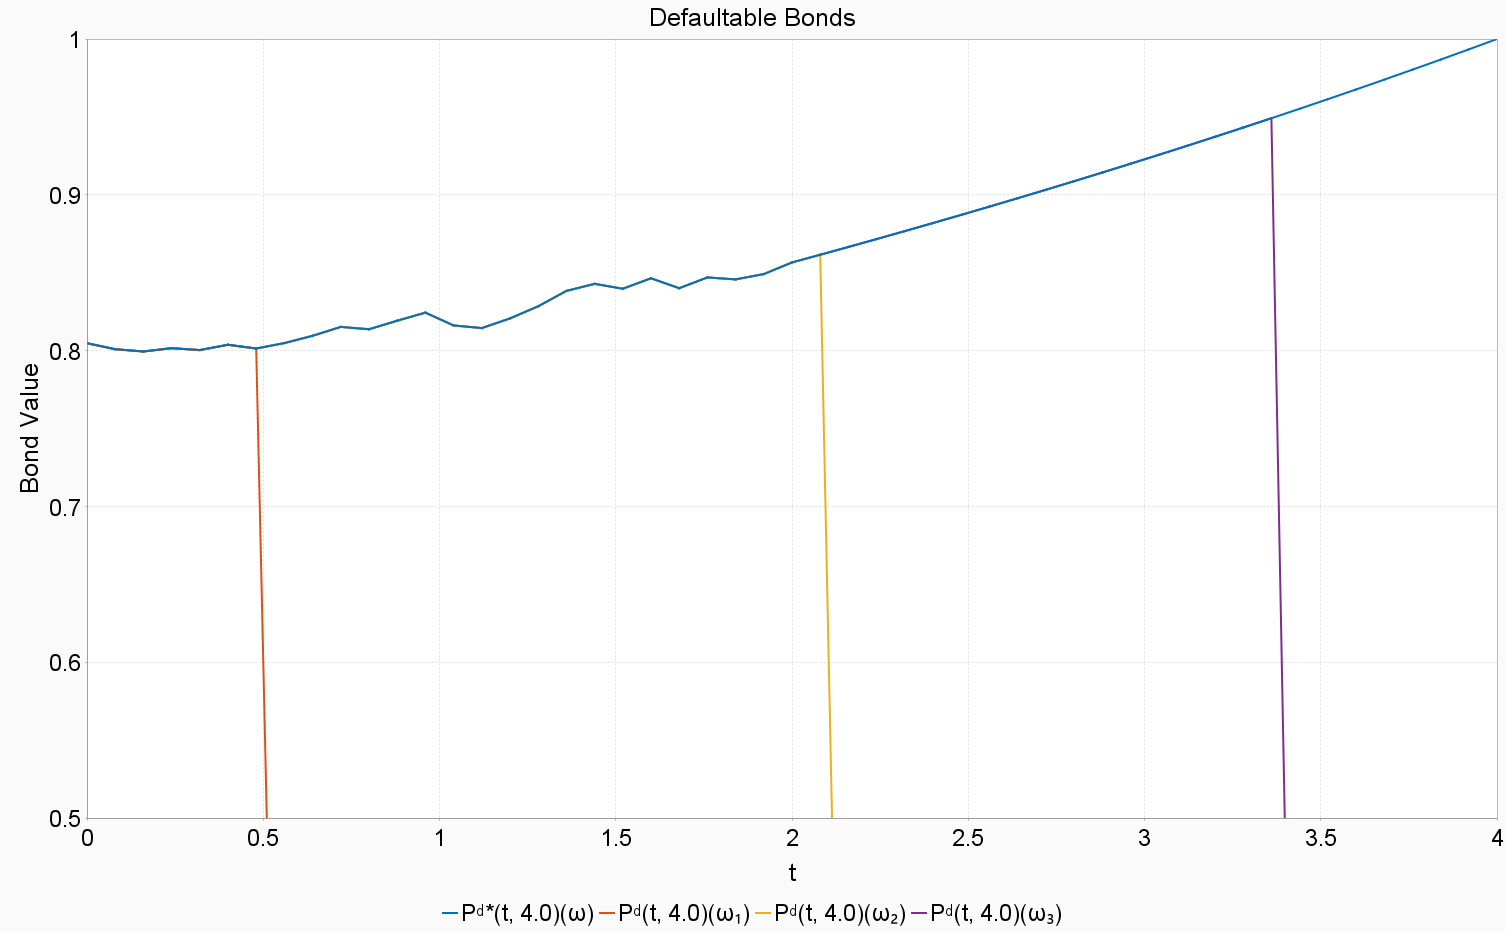
\includegraphics[width=\linewidth]{SurvivalProbability}
		\caption{Paths of $P^d$}
		\label{fig:survivalprobabilityvisualisation}
	\end{figure}
	\\In this example $\mathbb{G}$ captures only the path of $P^{d,*}(t; 4.0)$, which is equal for $\omega = \omega_1, \omega_2$ and $\omega_3$, while $P^d(t; 4.0)(\omega_1) \ne P^d(t; 4.0)(\omega_2) \ne P^d(t; 4.0)(\omega_3)$ for $t = 4.0$.
	\end{comment}
	\\Let us define a new value:
	\begin{definition}\label{def:totalsuvivalprob}
		Let $i \in \{1, ..., N\}$. We define the random variable $Q$ as
		\begin{align*}
			Q(T_i, \omega) = \prod_{j=1}^{i}q(T_j, \omega)
		\end{align*}
	\end{definition}
	While $Q$ in theory is not a probability, we can view it as the pathwise survival probability until $T_i$, if we have no information regarding the actual default state even at time $T_i$. Note that this is an \emph{interpretation} and the actual proof for this statement needs extra assumptions \color{red}[Attach proof for this?]\color{black}.\\
	What we actually prove in the next chapter is that the total survival probability until $T_i$ is given by the expectation of $Q$:
	\begin{align*}
		\mathbb{Q}^B\left(\{\tau > T_i\}\right) = \mathbb{E}^{\mathbb{Q}^B} \left[Q(T_i;\omega)\right]
	\end{align*}
	Let us rewrite the before derived/defined values in terms of $L$ and $L^d$:
	\begin{remark}
		Note that 
		\begin{align*}
			q(T_{i+1}, \omega) = \dfrac{1 + \Delta  T_i L_i(T_i)(\omega)}{1 + \Delta  T_i L^d_i(T_i)(\omega)}.
		\end{align*}
		Furthermore, with the definition of $q(T_i, \omega)$ one can rewrite $Q$ in terms of the numeraire $B(T_i)$ (corresponding to the Spot measure):
		\begin{align*}
			Q\left( T_{i+1}, \omega \right) = \dfrac{B(T_i)}{\prod_{k=0}^{i}(1 + \Delta T_k L^d_k(T_k)(\omega))} =: \dfrac{B(T_i)}{B^d(T_i)}.
		\end{align*}
		Note that $Q(T_i, \omega)$ is $\mathcal{G}_{T_{i-1}}$-measurable.
	\end{remark}
	The denominator in this equation can be seen as a "defaultable numeraire", which we define next:
	\begin{definition}
		We call $B^d$ given by:
		\begin{align*}
			B^d(t) = P^{d,*}(t;T_{m(t)+1}) \prod_{k=1}^{m(t)}\frac{1}{P^{d,*}(T_k;T_{k+1})} = P^{d,*}(t;T_{m(t)+1}) \prod_{k=1}^{m(t)}(1+\Delta T_k L^d_k(T_k))
		\end{align*}
		the \emph{defaultable numeraire}. 
	\end{definition}
	Due to $B^d$ not being a traded product, it is not a real numeraire. Hence there is not an equivalent martingale measure w.r.t. $B^d$ that we can use to price other products. And yet, we will see that the pricing formula for defaultable products is similar to a change of numeraires with $B^d$. Therefore, let us look at pricing in more detail.
	
	
	
	% -------- Pricing of credits with optionalities
	
	
	\pagebreak
	\section{Loans and Credit Option Pricing}\label{sec:pricing}
	A model is useless without a practical application for it. Hence we take a look at how to apply our results to pricing loans and credit options.\\
	Note here that the model is for use in numerical option pricing, so deriving prices in terms of an expectation over model primitives (directly simulated values or values that can be derived from these) is sufficient. We can then use Monte Carlo methods to approximate the expectation.\\
	For a start let us define our simulation filtration:
	\begin{definition}
		The filtration $\mathbb{F} := (\mathcal{F}_t)_{t\in\left[0,\tilde{T}\right]}$ is given by
		\begin{align*}
			\mathcal{F}_t := \sigma(U^k_t | k = 1, ..., m^d) \subset \mathcal{G}_t \quad \forall t \in  [0,\tilde{T}].
		\end{align*}
	\end{definition}
	Note that all model primitives are $\mathbb{F}$-adapted, as $\mathbb{F}$ is the filtration over the only simulated stochastic processes (in our case the Brownian Motion $U$). As mentioned before we are interested in pricing without simulating the default time $\tau$, which might be driven by other stochastic values. This means that $\tau$ is not necessarily a stopping time w.r.t. $\mathbb{F}$.
	
	\subsection{General Application}
	In this subsection, we derive a general pricing methodology before moving to specific products.\\
	A problem is that our model does not capture default. This is illustrated in \cref{fig:survivalprobabilityvisualisation}.
	\begin{figure}[h]
		\centering
		\includegraphics[width=\linewidth]{\fig{SurvivalProbability}}
		\caption{Paths of $P^d$}
		\label{fig:survivalprobabilityvisualisation}
	\end{figure}
	\\While the model simulates only paths of $P^{d,*}(t; T_i)$ (in the figure $P^{d,*}(t; 4.0)$), there are indefinitely many paths of $P^d(t;T_i)$ (in the figure $P^d(t; 4.0)(\omega_j)$ for $j \in \{1,2,3\}$) which satisfy
	\begin{align*}
		P^d(t;T_i) = P^{d,*}(t;T_i)(1 - J(t)),
	\end{align*} 
	but are not equal.\\
	We therefore use a trick and replace the default state $1-J(t)$ in all our pricing formulas with the random variable $Q$ that we defined in the previous chapter. \\
	To prove this works, assume a $T_i$-claim $X$ that has a payoff that is dependent on survival of the defaultable bonds. We can then use the pricing methodology described in te following lemma.
	\begin{lemma}\label{lm:pricingdefaultableclaims}
		Let $X$ be a payoff at $T_i \in \{T_1, ..., T_N\}$, with
		\begin{align*}
			X = X^S \mathbf{1}_{\{\tau(\omega) > T_i\}},
		\end{align*}
		where $X^S$ is the payoff conditional pre-default. Let $X^S$ be $\mathcal{F}_{T_i}$-measurable.\\
		Then the price at time $t=0$ is
		\begin{align*}
			\Pi^X = \mathbb{E}^{\mathbb{Q}^B}\left[ \frac{X^S}{B(T_i)} Q\left(T_i,\omega\right) \right].
		\end{align*}
	\end{lemma}
	Note that by construction $Q(T_i, \omega)$ is $\mathcal{F}_{T_i}$-measurable, which means, we have a price in terms of model primitives. Let us now prove this statement.
	\begin{proof} 
		For our proof we use following property of the conditional expectation extensively:
		\begin{align*}
			\mathbb{E}^{\mathbb{Q}^B}\left[Y\right] = \mathbb{E}^{\mathbb{Q}^B}\left[Y | A\right]\mathbb{Q}^B(A) + \mathbb{E}^{\mathbb{Q}^B}\left[Y | A^c\right]\mathbb{Q}^B(A^c) \tag{A}
		\end{align*}
		for any set $A \in \mathcal{G}$.\\
		For ease of notation we write $q(T_i):= q(T_i, \omega)$ and $Q(T_i):= Q(T_i, \omega)$. Note $B(T_0) = 1$. We have:
		\begin{align*}
			\Pi^X &=  \mathbb{E}^{\mathbb{Q}^B}\left[\frac{X^S}{B(T_i)} \mathbf{1}_{\{\tau(\omega) > T_i\}} \right]\\
			&=
			\mathbb{E}^{\mathbb{Q}^B}\left[\left.\frac{X^S}{B(T_i)} \mathbf{1}_{\{\tau(\omega) > T_i\}} \right| \{\tau > T_1\} \right]q(T_1) \tag{B}\\
			&=
			\mathbb{E}^{\mathbb{Q}^B}\left[\mathbb{E}^{\mathbb{Q}^B}_{\mathcal{G}_{T_1}}\left[\left.q(T_1)\frac{X^S}{B(T_i)} \mathbf{1}_{\{\tau(\omega) > T_i\}} \right| \{\tau > T_1\}\right] \right]\tag{C}\\
			&=
			\mathbb{E}^{\mathbb{Q}^B}\left[\mathbb{E}^{\mathbb{Q}^B}_{\mathcal{G}_{T_1}}\left[\left.q(T_1)\frac{X^S}{B(T_i)} \mathbf{1}_{\{\tau(\omega) > T_i\}} \right| \{\tau > T_2\}\right] q(T_2)\right]\\
			&=\mathbb{E}^{\mathbb{Q}^B}\left[\mathbb{E}^{\mathbb{Q}^B}_{\mathcal{G}_{T_2}}\left[\left.Q(T_2)\frac{X^S}{B(T_i)} \mathbf{1}_{\{\tau(\omega) > T_i\}} \right| \{\tau > T_2\}\right] \right]\\
			&=...\\
			&= \mathbb{E}^{\mathbb{Q}^B}\left[\mathbb{E}^{\mathbb{Q}^B}_{\mathcal{G}_{T_i}}\left[\left.Q(T_i)\frac{X^S}{B(T_i)} \mathbf{1}_{\{\tau(\omega) > T_i\}} \right| \{\tau > T_i\}\right] \right] \tag{D}\\
			&= \mathbb{E}^{\mathbb{Q}^B}\left[Q(T_i)\frac{X^S}{B(T_i)}\right],\tag{E}
		\end{align*}
		where (B) comes from (A) and (C) comes from the tower property and the fact that $q(T_1)$ is a constant. Then we repeat these steps until equation (D) always keeping in mind $q(T_j)$ is $\mathcal{G}_{T_i}$-measurable for all $j \le i$.
	\end{proof}
	\begin{remark}
		Note that in (E) of the proof we omitted the condition on $\{\tau > T_i\}$. This means that $X^S$ is independent of this set. We can make this assumption, w.l.o.g. because $X^S$ was only ever defined for this set. So we can basically "extend" it, such that it has the same distribution under $\{\tau \le T_i\}$, which makes it independent of these sets.
	\end{remark}
	This methodology can easily be extended to products where only parts of the payoff are dependent on survival and even where other parts are dependent on default:
	
	\begin{lemma}
		Let $X$ be a payoff at $T_i \in \{T_1, ..., T_N\}$, with
		\begin{align*}
			X = X^O + X^S \mathbf{1}_{\{\tau(\omega) > T_i\}} + X^D \mathbf{1}_{\{\tau(\omega) \le T_i\}},
		\end{align*}
		where the payoff $X^O$ is unconditional, $X^S$ is conditional pre-default and $X^D$ is conditional past-default and all are  $\mathcal{F}_{T_i}$-measurable.\\
		Then the price at time $t=0$ is
		\begin{align*}
			\Pi^X =& \mathbb{E}^{\mathbb{Q}^B}\left[ \frac{X^O}{B(T_i)} \right]
			+\mathbb{E}^{\mathbb{Q}^B}\left[ \frac{X^S}{B(T_i)} Q(T_i) \right] + \mathbb{E}^{\mathbb{Q}^B}\left[ \frac{X^D}{B(T_i)} \left(1 - Q(T_i)\right) \right].
		\end{align*}
	\end{lemma}
	\begin{proof}
		For the parts $X^O$ and $X^S$ the statement clear. For $X^D$ we have:
		\begin{align*}
			\mathbb{E}^{\mathbb{Q}^B}\left[ \frac{X^D}{B(T_i)} J(T_i) \right]
			&= \mathbb{E}^{\mathbb{Q}^B}\left[ \frac{X^D}{B(T_i)}\right] - \mathbb{E}^{\mathbb{Q}^B}\left[ \frac{X^D}{B(T_i)} \mathbf{1}_{\{\tau(\omega) > T_i\}} \right]\\
			&=\mathbb{E}^{\mathbb{Q}^B}\left[ \frac{X^D}{B(T_i)} \left(1 - Q(T_i)\right) \right]
		\end{align*}
		with the same arguments as in the lemma before.
	\end{proof}
	Lets re-evaluate the above equation with our expression for $Q$. One might notice that pricing defaultable products is similar to a change of numeraire with the defaultable numeraire: 
	\begin{align}\label{eq:defaultableclaimvaluation}
		\mathbb{E}^{\mathbb{Q}^B}\left[ \frac{X^S}{B(T_i)} Q(T_i) \right] =
		\mathbb{E}^{\mathbb{Q}^B}\left[ \frac{X^S}{B^d(T_i)} \right].
	\end{align}
	While this cannot hold up as a proof, it can be used as an intuitive explanation: we exchange the theoretical time value of future money with one that also accounts for default possibilities.\\
	With this expression it is also easy to derive an alternative numerical price for the defaultable zero-coupon bonds, by setting $X^S=1$:
	\begin{align*}
		P^d(0;T_i) = P^{d,*}(0;T_i) = \mathbb{E}^{\mathbb{Q}^B}\left[ \frac{1}{B^d(T_i)} \right]
	\end{align*}
	While we normally have the analytic value of $P^d(0, T_i)$ as an input value to our model (or at least calibrated from other input values), the numerical price can act as an error measurement for the model we create. Furthermore, we can later use it as a control variate in pricing, as it is done for the non defaultable model (see \cite{FriesBook}), which is beyond the scope of this thesis.\\
	We can also get a numerical expression for the total survival probability, because setting
	$X^S = B(T_i)$ and pricing the claim yields:
	\begin{align*}
		\Pi^X &= \mathbb{E}^{\mathbb{Q}^B}\left[ \frac{X^S}{B(T_i)} \mathbf{1}_{\{\tau(\omega) > T_i\}}\right] = \mathbb{E}^{\mathbb{Q}^B}\left[ \mathbf{1}_{\{\tau(\omega) > T_i\}}\right]
		= \mathbb{Q}^B(\{\tau > T_i\})\\
		&= \mathbb{E}^{\mathbb{Q}^B}\left[ Q(T_i)\right]
	\end{align*}
	Let us now extend this model. Assume a product is dependent on the survival of two different parties. For use in later sections we will call them debtor and  creditor.\\
	Such a claim is of the form
	\begin{align}\label{eq:claimtwopartysurvive}
		X = X^S\mathbf{1}_{\{\tau^d > T_i\}}\mathbf{1}_{\{\tau^c > T_i\}},
	\end{align}
	where $\tau^d$ is the default time of the debtor and $\tau^c$ that of the creditor.
	Before we go on to find the price of such a claim, let us first state an assumption for simplicity's sake:
	\begin{assumption}\label{as:counterpartiesareindependent}
		The default time of the debtor $\tau^d$ is independent of that the creditor $\tau^c$.
	\end{assumption}
	While this assumption is not realistic for all counter parties (the default of a big bank often triggers a wave of defaults of its clients \color{red}[Add source]\color{black}), %TODO: Add source
	we can assume that it is true for most.\\
	The price of such a claim can be found in the same way as above:
	\begin{lemma}\label{lem:creditordefPrice}
		Let \cref{as:counterpartiesareindependent} hold. The price for a $T_i$ claim with a payoff function as in \cref{eq:claimtwopartysurvive} can be computed by
		\begin{align*}
			\Pi^\Psi = \mathbb{E}^{\mathbb{Q}^B}\left[\dfrac{X^S}{B(T_i)}Q^d(T_i)Q^c(T_i)\right],
		\end{align*}
		where $Q^d$ and $Q^c$ are computed as given in \cref{def:totalsuvivalprob} from two separate defaultable LIBOR market models with the same underlying non-defaultable model.
	\end{lemma}
	Note that we now construct a totally new set of defaultable values: we have the defaultable LIBOR market model for the debtor with $P^{d^d,*}$, $L^{d^d}$ and their default time $\tau^d$ and we have a second defaultable model for the creditor and their values: $P^{d^c,*}$, $L^{d^c}$ and $\tau^c$. At the same time we still have the underlying non defaultable LIBOR market model.
	\begin{proof}
		For ease of notation let $A_j := \{\tau^d > T_j\} \cap\{\tau^c > T_j\}$ for all $j \in \{1, ..., N\}$.
		We follow exactly the proof of \cref{lm:pricingdefaultableclaims}, only we exchange $\mathbf{1}_{\{\tau > T_i\}}$ with $\mathbf{1}_{A_i}$:
		\begin{align*}
			\Pi^X &=  \mathbb{E}^{\mathbb{Q}^B}\left[\frac{X^S}{B(T_i)} \mathbf{1}_{A_i} \right]\\
		 	&=
		 	\mathbb{E}^{\mathbb{Q}^B}\left[\left.\frac{X^S}{B(T_i)} \mathbf{1}_{A_i} \right| A_1 \right]q^d(T_1)q^c(T_1)\tag{A}\\
		 	&=...\\
		 	&= \mathbb{E}^{\mathbb{Q}^B}\left[\mathbb{E}^{\mathbb{Q}^B}_{\mathcal{G}_{T_i}}\left[\left.Q^d(T_i)Q^c(T_i)\frac{X^S}{B(T_i)} \mathbf{1}_{A_i} \right| A_i \right]\right]\tag{B}
		\end{align*}
		where we get (A) from the independence of $\tau^d$ and $\tau^c$:
		\begin{align*}
		 	\mathbb{Q}^B\left(\{\tau^d > T_1\} \cap\{\tau^c > T_1\}\right) = q^d(T_1)q^c(T_1)
		\end{align*}
		and (B) in the same way as in the proof of \cref{lm:pricingdefaultableclaims}.
	\end{proof}
	
	
	With these formulas we now have an expression for claim prices in terms of an expectation over model primitives. We can therefore move to more specific products now.
	
	\subsection{General Loan Pricing}
	Let us first take a look what a loan is in general. "A loan is a sum of money that one or more individuals or companies borrow from banks or other financial institutions [...]. In doing so, the borrower incurs a debt, which he has to pay back with interest and within a given period of time."\cite{corpFinInst}.\\
	Hence a loan is nothing else than a fixed coupon bond, where the nominal $\mathcal{N}$ represents the debt and the coupons $c_i$ represent the interest.
	In the non defaultable case, "pricing" the loan is therefore nothing else than setting the coupons such that (we assume the same coupon tenor as LIBOR tenor):
	\begin{align}\label{eq:pricingnondefaultableloans}
		\mathcal{N} \mbeq \sum_{i=1}^{N}c_i P(0;T_i) + \mathcal{N}P(0;T_N)
	\end{align}
	\begin{remark}\label{rem:nativecouponsforloans}
		Setting 
		\begin{align*}
			c_i = \mathcal{N}\Delta T_iL_i(0)
		\end{align*}
		satisfies \cref{eq:pricingnondefaultableloans} and therefore yields a valid loan.
	\end{remark}
	\begin{proof}
		We have 
		\begin{align*}
			\Delta T_iL_{i-1}(0) = \frac{P(0;T_{i-1})}{P(0;T_{i})} - 1
		\end{align*}
		Inserting in \cref{eq:pricingnondefaultableloans} yields (note $P(0;T_0) = 1$):
		\begin{align*}
			\sum_{i=1}^{N}\mathcal{N}\Delta T_iL_i(0) P(0;T_i) + \mathcal{N}P(0;T_N) \\
			=\sum_{i=1}^{N}\mathcal{N}(\frac{P(0;T_{i-1})}{P(0;T_{i})} - 1) P(0;T_i) + \mathcal{N}P(0;T_N)\\
			= \sum_{i=1}^{N}\mathcal{N}(P(0;T_{i-1}) - P(0;T_{i})) + \mathcal{N}P(0;T_N) = \mathcal{N}
		\end{align*}
	\end{proof}
	Let us look at the defaultable case:
	\begin{lemma}
		The price of a coupon paying bond which has defaultable cashflows is:
		\begin{align*}
			\mathcal{N} = \sum_{i=1}^{N}c_i P^{d,*}(0;T_i) + \mathcal{N}P^{d,*}(0;T_N)
		\end{align*}
	\end{lemma}
	\begin{proof}
		Let $c\in \mathbb{R}$ be constant. Then for $i \in \{1, ..., N\}$:
		\begin{align*}
			&\mathbb{E}^{\mathbb{Q}^B}\left[\frac{c\;\mathbf{1}_{\left\{\tau(\omega) > T_{i} \right\}}}{B(T_i)}\right] = c \; \mathbb{E}^{\mathbb{Q}^B}\left[ 
			\frac{P^d(T_i;T_i)}{B(T_i)} \right]\\
			&= c \; P^d(0;T_i) = c \; P^{d,*}(0;T_i).
		\end{align*}
		Replacing $c$ with $c_i$, $\mathcal{N}$ repectively, and taking the sum yields the statement.
	\end{proof}
	A loan, where the debtor is defaultable hence must satisfy:
	\begin{align*}
		\mathcal{N} \mbeq \sum_{i=1}^{N}c_i P^{d,*}(0;T_i) + \mathcal{N}P^{d,*}(0;T_N)
	\end{align*}
	We again have a natural solution to this equation. With the same arguments as for \cref{rem:nativecouponsforloans} we find that setting
	\begin{align*}
		c_i = \mathcal{N}\Delta T_iL^d_i(0)
	\end{align*}
	yields a valid loan.\\
	Note that for a simple loan it does not matter if the creditor is defaultable, because they have no debt w.r.t. the loan after $t=0$ and in case of their default the pending claim would still be collected.\\
	Let us take a look at a future on defaultable loans, or rather a future on a defaultable coupon paying bond. 
	Remember that in contrast to an option a future brings the obligation to enter into an agreement.
	Hence from the debtors point of view we have a payoff function
	\begin{align}\label{eq:loanForward}
		\Psi(T_s) = \left(\mathcal{N} - \sum_{i=s+1}^{N}c_iP^{d,*}(T_s; T_i)\right)\mathbf{1}_{\{\tau > T_s\}}
	\end{align}
	where $T_s$ is the start time of the bond and for ease of notation the terminal coupon $c_N$ includes the terminal payment of the nominal $\mathcal{N}$.\\
	This payoff function gives us a direct approach to price the product:
	\begin{lemma}\label{lm:simpledefcouponbondforward}
		A $T_s$ claim with a payoff function as in \cref{eq:loanForward} has the price
		\begin{align*}
			\Pi^\Psi &= \mathcal{N}P^d(0;T_s) - \sum_{i=s+1}^{N}c_iP^{d}(0; T_i)\\
			&= \mathcal{N}P^{d,*}(0;T_s) - \sum_{i=s+1}^{N}c_iP^{d,*}(0; T_i)
		\end{align*}
		at $t=0$.
	\end{lemma}
	\begin{proof}
		We have:
		\begin{align*}
			\Pi^\Psi &= \mathbb{E}^{\mathbb{Q}}\left[\dfrac{\left(\mathcal{N} - \sum_{i=s+1}^{N}c_iP^{d,*}(T_s; T_i)\right)\mathbf{1}_{\{\tau > T_s\}}}{B(T_s)}\right]\\
			&=\mathcal{N}\mathbb{E}^{\mathbb{Q}}\left[\dfrac{P^d(T_s;T_s)}{B(T_s)}\right] - \sum_{i=s+1}^{N} c_i \mathbb{E}^{\mathbb{Q}}\left[\dfrac{P^d(T_s;T_i)}{B(T_s)}\right]\\
			&= \mathcal{N}P^d(0;T_s) - \sum_{i=s+1}^{N} c_i P^d(0;T_i)
		\end{align*}
	\end{proof}
	To gain an initial price of zero one can set the coupons as done before:
	\begin{align*}
		c_i = \mathcal{N}\Delta T_iL^d_i(0), \quad c_N = \mathcal{N}\left(1 + \Delta T_iL^d_i(0)\right).
	\end{align*}
	Let us rewrite the same price as discussed in \cref{lm:simpledefcouponbondforward} for a numerical valuation instead of an analytic one:
	\begin{align*}
		\Pi^\Psi &= \mathbb{E}^{\mathbb{Q}^B}\left[\dfrac{\mathcal{N} - \sum_{i=s+1}^{N}c_iP^{d,*}(T_s; T_i)}{B(T_s)}Q(T_s)\right].
	\end{align*}
	Here one can see that the forward has two main stochastic cost drivers: 
	\begin{itemize}
		\item The default probability \emph{past} maturity time, which has a positive relation to the price: if the default probability rises, $P^{d,*}(T_s;T_i)$ decreases, which drives the price up.
		\item The default probability \emph{before} maturity time, which has a negative relation to the price intensity: if the default probability rises, $Q(T_s)$ decreases, which lowers the absolute value of the price (as $0 < Q(T_s) < 1$).
	\end{itemize}
	In the past example default of the creditor did not matter, but in this case actually the future contract depends on their survival. Hence creditor default possibility does indeed change the payoff
	\begin{align}\label{eq:loanForwardCreditorDefaultable}
		\Psi(T_s) = \left(\mathcal{N} - \sum_{i=s+1}^{N}c_iP^{d^d,*}(T_s; T_i)\right)\mathbf{1}_{\{\tau^d > T_s\}}\mathbf{1}_{\{\tau^c > T_s\}}.
	\end{align}
	and hence also the price of such a product:
	\begin{lemma}
		Let \cref{as:counterpartiesareindependent} hold. The price for a product with a payoff as in \cref{eq:loanForwardCreditorDefaultable} at $t=0$ is:
		\begin{align*}
			\Pi^\Psi &= \mathbb{E}^{\mathbb{Q}^B}\left[\dfrac{\mathcal{N} - \sum_{i=s+1}^{N}c_iP^{d^d,*}(T_s; T_i)}{B(T_s)}Q^d(T_s)Q^c(T_s)\right]\\
			&= \mathbb{E}^{\mathbb{Q}^B}\left[\dfrac{\mathcal{N} - \sum_{i=s+1}^{N}c_iP^{d^d,*}(T_s; T_i)}{B^{d^d}(T_s)}Q^c(T_s)\right]
		\end{align*}
	\end{lemma}
	\begin{proof}
		Follows directly from \cref{lem:creditordefPrice}.
	\end{proof}
	\begin{figure}[h]
		\centering
		\includegraphics[width=0.7\linewidth]{\fig{ValuationCouponBondForwards}}
		\caption[Valuation of Forwards on Coupon Bonds]{Valuation of Forwards on Coupon Bonds}
		\label{fig:valuationcouponbondforwards}
	\end{figure}
	It is easy to see that the price of a coupon bond forward, which considers both parties to be defaultable is less intense (i.e. it decreases the absolute value of the price more) than that, which only considers the debtor to be defaultable. In \cref{fig:valuationcouponbondforwards} one can also see that the difference increases the further maturity is away.
	
	
	\subsection{Credit Options}
	In the last subsection we considered pricing loans and loan forwards. Essentially cash flow that is set in stone (with the exception of default). 
	Now let us consider more intriguing products which bring an optionality with them:
	We start with a simple put option on a coupon bond (note that we work a lot with coupon bonds as to their equivalence with a loan). 
	\begin{remark}
		A put option on a coupon paying bond, with maturity $T_s$ and strike price $\mathcal{N}$ where the debtor/payer is defaultable has the payoff function
		\begin{align}\label{eq:couponputoption}
			\Psi(T_s) =\left(\mathcal{N} - \sum_{i=s+1}^{N}c_iP^{d,*}(T_s; T_i)\right)^+\mathbf{1}_{\{\tau > T_s\}}
		\end{align}
		where $\left(\cdot\right)^+ := \max(0, \cdot)$.
	\end{remark}
	We can numerically compute the price.
	\begin{lemma}
		A claim with a payoff function as in \cref{eq:couponputoption} has the price:
		\begin{align*}
			\Pi^\Psi =\mathbb{E}^{\mathbb{Q}^B}\left[\dfrac{\left(\mathcal{N} - \sum_{i=s+1}^{N}c_iP^{d,*}(T_s; T_i)\right)^+}{B^d(T_s)}\right]
		\end{align*}
	\end{lemma}
	\begin{proof}
		Directly follows from \cref{lm:pricingdefaultableclaims}.
	\end{proof}
	Also this product can be extended to both counter parties being defaultable: the debtor and the creditor.\\
	The adjusted formulas are
	\begin{align*}
		\Psi(T_s) =\left(\mathcal{N} - \sum_{i=s+1}^{N}c_iP^{d^d,*}(T_s; T_i)\right)^+\mathbf{1}_{\{\tau^d > T_s\}}\mathbf{1}_{\{\tau^c > T_s\}}
	\end{align*}
	for the payoff and 
	\begin{align*}
		\Pi^\Psi =\mathbb{E}^{\mathbb{Q}^B}\left[\dfrac{\left(\mathcal{N} - \sum_{i=s+1}^{N}c_iP^{d^d,*}(T_s; T_i)\right)^+}{B^{d^d}(T_s)}Q^c(T_s)\right]
	\end{align*}
	for pricing. A proof is omitted as it is trivial.\\
	A more advanced product is a cancellable loan. We start with the case, where one can cancel the loan at a single time point $T_k$ for $k \in \{1, ... N-1\}$.\\
	Consider the cash flow of such a product from the debtors point of view:
	We get the nominal $\mathcal{N}$ at the start of the loan. Then we pay coupons each tenor until $T_k$. If we cancel the loan, we have to pay the redemption $\tilde{R}$, otherwise we keep paying coupons until the end of the loan.
	\begin{figure}[h]
		\centering
		\makebox[\textwidth][c]{%
			\subfloat{\scalebox{0.4}{\includegraphics{\fig{CancellableLoan}}}}
			\quad
			\subfloat{\scalebox{0.4}{\includegraphics{\fig{LoanAndPutOption}}}}
		}
		\caption[Cashflow of a cancellable loan and its splitting into two products]{Cashflow of a cancellable loan and its splitting into two products}
		\label{fig:cancellableloan}
	\end{figure}
	\\To derive a price for this product, we split the cash flow in two parts: a  loan and a put option on a loan, as visualized in \cref{fig:cancellableloan}. 
	The option is then treated as single cash flow in terms of the price, which leads us to a payoff of (note, we again only consider debtor default):
	
	\begin{center}
		\begin{tabular}{cl}
			$\mathcal{N}$ & at $T_0$, \\
			$-c_i\mathbf{1}_{\{\tau > T_i\}}$ 		  & at $T_i$ for $i \in \{1, ..., N\}$, \\
			$\left(\sum_{j=k+1}^{N}c_jP^{d,*}(T_k;T_j) - \tilde{R}\right)^+\mathbf{1}_{\{\tau > T_k\}}$ 
			& at $T_k$.
		\end{tabular}
	\end{center}
	Note that if $\left(\sum_{j=k+1}^{N}c_jP^{d,*}(T_k;T_j) - \tilde{R}\right) > 0$ at $T_k$, the debtor could get a new loan on the nominal $\tilde{R}$ for better conditions then the initial one.\\
	From there it is easy to compute the price:
	\begin{align}\label{eq:priceofcancellableloan}
		\mathcal{N} -\sum_{i=1}^{N}c_iP^{d,*}(0;T_i) +  \mathbb{E}^{\mathbb{Q}^B}\left[\dfrac{\left(\sum_{j=k+1}^{N}c_jP^{d,*}(T_k;T_j) - \tilde{R}\right)^+}{B^d(T_k)}\right]
	\end{align}
	
	\begin{remark}
		One can also construct the cash flows for the cancellable loan from a loan and a call option on a loan:

		\begin{center}
			\begin{tabular}{cl}
				$\mathcal{N}$ & at $T_0$, \\
				$-c_i\mathbf{1}_{\{\tau > T_i\}}$ 		  & at $T_i$ for $i \in \{1, ..., k\}$, \\
				$-\tilde{R}\mathbf{1}_{\{\tau > T_k\}}$  & at $T_k$ and\\
				$\left(\tilde{R} - \sum_{j=k+1}^{N}c_jP^{d,*}(T_k;T_j) \right)^+\mathbf{1}_{\{\tau > T_k\}}$ 
				& at $T_k$.
			\end{tabular}
		\end{center}
		
		For any $c_i, \mathcal{N}, \tilde{R} \in \mathbb{R}$ for $i \in \{1, ..., N\}$ this will yield the same price formula as \cref{eq:priceofcancellableloan}.
	\end{remark}
	\begin{proof}
		This can be trivially derived from the relation:
		\begin{align*}
			&\mathbb{E}^{\mathbb{Q}^B}\left[\dfrac{\left(\sum_{j=k+1}^{N}c_jP^{d,*}(T_k;T_j) - \tilde{R}\right)^+}{B^d(T_k)}\right]\\
			&\;= \mathbb{E}^{\mathbb{Q}^B}\left[\dfrac{\left(\tilde{R} - \sum_{j=k+1}^{N}c_jP^{d,*}(T_k;T_j)\right)^+}{B^d(T_k)}\right]
			+ \mathbb{E}^{\mathbb{Q}^B}\left[\dfrac{\sum_{j=k+1}^{N}c_jP^{d,*}(T_k;T_j) - \tilde{R}}{B^d(T_k)}\right]\\
			&\;= \mathbb{E}^{\mathbb{Q}^B}\left[\dfrac{\left(\tilde{R} - \sum_{j=k+1}^{N}c_jP^{d,*}(T_k;T_j)\right)^+}{B^d(T_k)}\right]
			+\sum_{j=k+1}^{N}c_jP^{d,*}(0;T_j) - \tilde{R}P^{d,*}(0;T_k)
		\end{align*}
	\end{proof}
	Let us look at how to set the starting value of the cancellable loan to zero.
	We have to set the coupons and $\tilde{R}$ such that:
	\begin{align*}
		\mathcal{N} + \Pi^\Psi \mbeq \sum_{i=1}^{N}c_iP^{d,*}(0;T_i),
	\end{align*}
	where $\Pi^\Psi$ is the price of a put option on a coupon bond with maturity $T_k$ and strike $\tilde{R}$, i.e.
	\begin{align*}
		\Pi^\Psi = \mathbb{E}^{\mathbb{Q}^B}\left[\dfrac{\left(\sum_{j=k+1}^{N}c_jP^{d,*}(T_k;T_j) - \tilde{R}\right)^+}{B^d(T_k)}\right]
	\end{align*}
	Note that it is easiest to distribute the value of $\Pi^\Psi$ on the first $k$ coupons, as $\Pi^\Psi$ itself is influenced by the later ones.
	Hence we can set the later coupons as done before and distribute the accrued price of $\Pi^\Psi$ to the earlier ones: 
	\begin{align*}
		c_i &= \mathcal{N} \Delta T_i L^d_i(0) + \frac{\Pi^\Psi}{k P^{d,*}(0;T_i)} \quad &\text{for } i \in \{1,...,k\}\\
		c_i &= \mathcal{N} \Delta T_i L^d_i(0) \quad &\text{for } i \in \{k+1,..., N -1\}\\
		c_i &= \mathcal{N} \left(\Delta T_i L^d_i(0) + 1\right) \quad &\text{for } i = N
	\end{align*}
	Generally the redemption $\tilde{R}$ can be set arbitrarily and the price formula will hold. However, \color{red}it is good practice to \color{black} set it to the price of the remaining nominal (which is not payed back through the coupons until $T_k$) plus a penalty $p\in \mathbb{R}$:
	\begin{align*}
		\tilde{R} = \sum_{j=k+1}^{N}c_j \frac{P^{d,*}(T_0;T_j)}{P^{d,*}(T_0;T_k)} + p
	\end{align*}
	%TODO: What is the price for both parties defaultable
	
	
	Let us generalize this product for the possibility to cancel at any time past $T_k$ for a fixed $k \in \{1,...,N-1\}$.
	Note that in this case the redemption $\tilde{R}_t$ would depend on the cancel time, but still be deterministic. Then the adjusted cash flow is
	
	\begin{center}
		\begin{tabular}{cl}
			$\mathcal{N}$ & at $T_0$, \\
			$-c_i\mathbf{1}_{\{\tau > T_i\}}$ 		  & at $T_i$ for $i \in \{1, ..., N\}$, \\
			$\left(\sum_{j=m(\nu)+1}^{N}c_jP^{d,*}(\nu;T_j) - \tilde{R}_\nu\right)\mathbf{1}_{\{\tau > \nu\}}$
			& at $\nu$,
		\end{tabular}
	\end{center}
	
	where $\nu = \nu(\omega)$ is the stopping time:
	\begin{align*}
		\nu(\omega) = \min\left(t\in \left[T_k,T_N\right[ \;\left| \;\left(\sum_{j=m(t)+1}^{N}c_jP^{d,*}(t;T_j) - \tilde{R}_t\right) > 0\right. \right) \wedge T_N
	\end{align*}
	Hence this has the form of an American option, where we can choose to exercise the option in the time interval $\left[T_k,T_N\right]$. As always the price can be obtained by taking the discounted expectation:	
	\begin{align*}
		\mathcal{N} -\sum_{i=1}^{N}c_iP^{d,*}(0;T_i) +  \mathbb{E}^{\mathbb{Q}^B}\left[\dfrac{\left(\sum_{j=m(\nu)+1}^{N}c_jP^{d,*}(\nu;T_j) - \tilde{R}_\nu\right)}{B^d(\nu)}\right].
	\end{align*}
	As $\nu$ is only dependent on $\mathbb{F}$-adapted values, it is also a value in terms of model primitives, which makes it usable to us.
	
	\subsection{Introducing Behavioral Aspects}
	Let us spin our model a bit further. Until now we have assumed that all market participants have a perfect overview of the market (captured by the filtration $\mathbb{G}$). Furthermore we assumed that debtors always act in an optimized manner (exercise the option if it has a positive value). While big companies may have implemented ways such that these are feasible assumptions, this is far from realistic for small market participants such as private people.\\
	A study from 2021 from Germany asked people how to best spend €1,000 given two options: making a special repayment of an existing loan of theirs, which charges 5 \% interest or invest in a fixed coupon bond with 3 \% interest and maturity of 3 years \cite{finKnowledgeStudy}.
	The results showed that only 60 \% of the participants would make the special repayment. 15 \% stated that they did not know the answer, 13 \% thought both options were equally good and 12 \% would rather buy the coupon bond \cite{finKnowledgeStudy}.\\
	% Not only knowing when to cancel, but also motivation is something to take into account when dealing with private debtors: 
	This shows that the assumption of optimal exercising for cancellable loans is an idealization and hence for fair pricing models we need to adjust for this deficit.
	
	\begin{remark}
		Note that in general (non-defaultable) option pricing an adjustment would generate an arbitrage possibility, because small market participants could buy cheap options and resell them to big companies at a higher price, without any risk.\\
		However, a cancellable loan is not transferable (the defaultable LIBOR models are calibrated to the individual client), meaning it also can not be resold. This closes the arbitrage possibility.
	\end{remark}
	
	How do we inject such a behavioral aspect in our valuation formula? We could construct a stochastic model which simulates the exercising of a market participant. However, we already omitted modeling the default time for the simple reason of computational cost and modeling behavior would require at least the same amount of computing power.\\
	Hence we try a simpler approach: we apply a so called deterministic shadow barrier $\tilde{S}_t$, for each $t \in \left[T_k,T_N\right]$, which leads to a different cash flow:
	
	\begin{center}
		\begin{tabular}{cl}
			$\mathcal{N}$ & at $T_0$, \\
			$-c_i\mathbf{1}_{\{\tau > T_i\}}$ 		  & at $T_i$ for $i \in \{1, ..., N\}$, \\
			$\left(\sum_{j=m(\nu)+1}^{N}c_jP^{d,*}(\nu;T_j) - \tilde{R}_\nu - \tilde{S}_\nu\right)\mathbf{1}_{\{\tau > \nu\}}$
			& at $\nu$,
		\end{tabular}
	\end{center}
	
	Generally one can see $\tilde{S}_t$ as the profit it takes, until the debtor would be motivated enough to exercise the option. The price calculation is equivalent to before, only we exchange $\tilde{R}_\nu$ for $\tilde{R}_\nu + \tilde{S}_\nu$:
	\begin{align*}
		\mathcal{N} -\sum_{i=1}^{N}c_iP^{d,*}(0;T_i) +  \mathbb{E}^{\mathbb{Q}^B}\left[\dfrac{\left(\sum_{j=m(\nu)+1}^{N}c_jP^{d,*}(\nu;T_j) - \tilde{R}_\nu - \tilde{S}_\nu\right)}{B^d(\nu)}\right].
	\end{align*}
	% TODO: Add a plot of a European cancellable loan, an American one and the Shadow barrier equivalents.
	%TODO: Warn about relending the money!
	
	
	
	
	% -------- Implementation of the main model ------------------
	
	
	\pagebreak
	\section{Numerical Specification}\label{sec:numerical}
	The implementation of the described concepts are a crucial part of this thesis.\\
	We use Java, which is a purely object oriented programming language, for having a good  code readability while still performing very well. We assume a basic knowledge in Java.
	As build system we use Maven.\\
	Before we can jump into any code, though, we need to describe ways to discretize a stochastic process.
	
	\subsection{Numerical Schemes for Stochastic Processes}
	In this chapter we introduce ways to approach the simulation of stochastic processes described by SDEs. These numerical schemes can also be found in \cite{kloedenSchemes}, which is also the main source of this section.\\
	As basis for the schemes we have a known SDE for a $n$-dimensional stochastic process $X=(X_t)_{t\in [0,\tilde{T}]}$ that we want to simulate:
	\begin{align}
		\begin{aligned}\label{eq:schemeGoalSDE}
		dX_t &= \mu(t, X_t)dt + \sigma(t, X_t) \cdot dU_t,\\
		X_0 &= x,
		\end{aligned}
	\end{align}
	where $U$ is a $d$-dimensional standard Brownian Motion, $\mu: [0,\tilde{T}] \times \mathbb{R}^n \rightarrow \mathbb{R}^n$ and $\sigma: [0,\tilde{T}] \times \mathbb{R}^n \rightarrow \mathbb{R}^{n \times d}$ are functions and $x \in \mathbb{R}^n$.\\
	Let us start with the well-known Euler or Euler-Maruyama scheme:
	\begin{definition}\label{def:eulerscheme}
		Let $X=(X_t)_{t\in [0,\tilde{T}]}$ be as above in (\ref{eq:schemeGoalSDE}).\\
		Furthermore let $m \in \mathbb{N}$, $(t_i)_{i\in \{0, ..., m\}}$, where $0=t_0 < t_1 < ... < t_m=\tilde{T}$.\\
		Then we call the discrete process $\hat{X} = (\hat{X}_{t_i})_{i \in \{0, ..., m\}}$, given by
		\begin{align*}
			\hat{X}_{t_0} &= x,\\
			\hat{X}_{t_{i+1}} &= \hat{X}_{t_{i}} + \mu(t_i, \hat{X}_{t_{i}})\Delta t_i + \sigma(t_i, \hat{X}_{t_{i}}) \cdot \Delta U_{t_i},
		\end{align*}
		where $i \in \{0, ..., m-1\}$, an \emph{Euler-Maruyama scheme of $X$}.
	\end{definition}
	
	The Euler-Maruyama scheme takes the concept of approaching deterministic integrals and applies it on stochastic integrals. While this works quite well for constant and deterministic factor loadings $\sigma(t_i, x) = \sigma(t_i)$ \color{red}[Add source]\color{black} %TODO: Add source
	, it has a weakness for stochastic factor loadings.\\
	An improvement would be the Milstein scheme as described in \cite{kloedenSchemes}, but due to its correction term, which gets fairly complicated for higher dimensional Brownian motions, it is not well suited for our purpose.
	\begin{comment}
	An improvement is the Milstein scheme:
	\begin{definition}\label{def:milsteinscheme}
		Let again $X=(X_t)_{t\in [0,\tilde{T}]}$ be as above in (\ref{eq:schemeGoalSDE}) and $m \in \mathbb{N}$, $(t_i)_{i\in \{0, ..., m\}}$, where $0=t_0 < t_1 < ... < t_m=\tilde{T}$.\\
		Then we call the discrete process $\hat{X} = (\hat{X}_{t_i})_{i \in \{0, ..., m\}}$, given by
		\begin{align*}
			\hat{X}_{t_0} =&\; x,\\
			\hat{X}^l_{t_{i+1}} =&\; \hat{X}^l_{t_{i}} + \mu(t_i, \hat{X}_{t_{i}})\Delta t_i + \sigma(t_i, \hat{X}_{t_{i}}) \cdot \Delta U_{t_i}\\
			&+ \frac{1}{2}\sum_{k=1}^{d}\sigma_k(t_i, \hat{X}_{t_i})(\partial_{x^k}\sigma_l)(t_i, \hat{X}_{t_i})((\Delta U^k_{t_i})^2 - \Delta t_i),
		\end{align*}
		where $i \in \{0, ..., m-1\}$ and $l \in \{1, ..., n\}$, a \emph{Milstein scheme of $X$}.
	\end{definition}
	This gives an improvement due to the correction term at the end. We can also easily see that if $\sigma$ is independent of $X_t$ the Milstein is equal to the Euler-Maruyama scheme.\\\end{comment}
	Instead we consider the functional Euler Scheme:
	\begin{definition}\label{def:funceulerscheme}
		Let $X=(X_t)_{t\in [0,\tilde{T}]}$ be as above in (\ref{eq:schemeGoalSDE}).\\
		Let $Y=(Y_t)_{t\in [0,\tilde{T}]}$ be defined as $Y_t = f(t, X_t) \quad \forall t\in [0,\tilde{T}]$ for a $2$-times differentiable function $f: [0,\tilde{T}] \times \mathbb{R}^n \rightarrow \mathbb{R}^k$ and $k \in \mathbb{N}$.\\
		Let $m \in \mathbb{N}$, $(t_i)_{i\in \{0, ..., m\}}$, where $0=t_0 < t_1 < ... < t_m=\tilde{T}$. Let  $\hat{X} = (\hat{X}_{t_i})_{i \in \{0, ..., m\}}$ be an Euler-Maruyama scheme of $X$.\\
		Then we call the discrete process $\hat{Y} = (\hat{Y}_{t_i})_{i \in \{0, ..., m\}}$, given by
		\begin{align*}
			\hat{Y}_{t_i} &= f(t,\hat{X}_{t_i}),
		\end{align*}
		where $i \in \{0, ..., m\}$, a \emph{functional Euler scheme of $Y$}.
	\end{definition}
	This scheme performs well in situations, where the factor loadings of $X$ are less dependent on $X$, than the factor loadings of $Y$ are on $Y$.\\
	It is also very useful, if $f$ preserves a property of $Y$ which otherwise might be lost through the numerical error of the other schemes (such as staying in a certain domain).\\
	Considering this, the functional Euler scheme is great for the approximation of log-normal processes, as it cancels a part of the numerical error due to the dependency of the factor loadings on the approximated process and at the same time it preserves its positivity.\\
	\begin{figure}[h]
		\centering
		\includegraphics[width=0.8\linewidth]{\fig{Schemes_DirectCompare}}
		\caption[Comparison of Numerical Schemes for a Geometric Brownian Motion]{Comparison of Numerical Schemes for a Geometric Brownian Motion}
		\label{fig:schemesdirectcompare}
	\end{figure}
	In \cref{fig:schemesdirectcompare} we can see a direct comparison of the schemes for two different paths of a geometric Brownian motion, i.e. $X_t = X_0\exp((\mu - 0.5 \sigma^2) t + \sigma W_t)$, where $X_0=0.1$, $\mu=-0.1$ and $\sigma=0.7$. As time discretization we chose $\Delta t = 0.2$.\\
	In this case the functional Euler scheme generates exact paths, which do not have any numeric error from discretizing the SDE.
	We see that the Euler scheme portrays a numerical error that is quite extensive at certain times. One path of the Euler scheme even reaches a value below zero, while the dynamics of the geometric Brownian motion are such that this should be impossible. It is worth to note, however, that the time discretization is chosen quite rough for demonstration purposes.\\
	%TODO Adjust the following sentece:
	To also prove that the schemes work analytically, we define some convergence rates as in \cite{kloedenSchemes}:
	\begin{definition}
		Let $\hat{X}^{\delta}$ be a time-discrete scheme for the approximation of a process $X$, where $\delta$ is the maximum time difference between approximations, i.e. $\delta=\max\left\{t_i-t_{i-1} | i\in \{1,...,m\}\right\}$.\\
		Then we say that $\hat{X}^{\delta}$ converges strongly to $X$ if:
		\begin{align*}
			\lim\limits_{\delta \downarrow 0} \mathbb{E}\left[\left|X_{\tilde{T}} - \hat{X}^{\delta}_{\tilde{T}} \right|\right] = 0.
		\end{align*}
		We say that $\hat{X}^{\delta}$ converges strongly with order $\gamma > 0$ to $X$ if $\exists C > 0$ and a $\delta_{max}$ such that
		\begin{align*}
			\mathbb{E}\left[\left|X_{\tilde{T}} - \hat{X}^{\delta}_{\tilde{T}} \right|\right] \le C\delta^\gamma
		\end{align*}
		for all $\delta \in \left]0,\delta_{max}\right[$.
	\end{definition}
	It is well known that the Euler scheme fulfills the  following properties:
	\begin{lemma}
		Let $X$ be the solution of \cref{eq:schemeGoalSDE}.
		Let furthermore 
		\begin{align*}
			|\mu(t,x) - \mu(t,y)| + |\sigma(t,x) - \sigma(t,y)| &\le K_1 |x - y|,\\
			|\mu(t,x)| + |\sigma(t,x)| &\le K_2(1+|x|),\\
			|\mu(t,x) - \mu(s,x)| + |\sigma(t,x) - \sigma(s,x)| &\le K_3 (1+|x|) |t - s|^{\frac{1}{2}}
		\end{align*}
		for all $s,t \in \left[0,\tilde{T}\right]$ and $x,y\in \mathbb{R}^n$ for some constants $K_1, K_2, K_3 \in \mathbb{R}$.
		Then the Euler scheme given in \cref{def:eulerscheme} converges strongly to $X$ with order $\frac{1}{2}$.
	\end{lemma}
	\begin{proof}
		See \cite{kloedenSchemes}, pp. 342.
	\end{proof}
	
	
	\subsection{The finMath Library}
	We can now start to look at the actual implementation.\\
	As a starting point for the code base we use the finMath Library of Prof. Christian Fries.\\
	The finMath library is written in Java and provides interfaces and classes for the use in stochastics and financial mathematics.\\
	In this section we take a look at the ones that are most frequently used by our code. For a more thorough description one can use the website of the finMath library \cite{finmathWebsite}, which is also our main source for this section.
	
	\subsubsection*{RandomVariable}
	As one can tell from the name, \texttt{RandomVariable} is an interface for working with stochastic values, hence it is the basis for Monte Carlo methods. Operator overloading is not possible in Java so the workaround is to have methods that represent these operations, which is what \texttt{RandomVariable} declares.
	Taking the expectation (the mean) and the variance is also supported. A nice feature is a \texttt{RandomVariableFactory}, which handles all creations of a \texttt{RandomVariable}.
	
	\subsubsection*{ProcessModel}
	The \texttt{ProcessModel} interface is the finMath equivalent of an SDE. It specifies that any implementation has methods for getting the initial state, the drift and the factor loadings.
	
	\lstinputlisting[caption={The  \texttt{ProcessModel} interface (some methods are ommitted)}, label={lst:javaCode1}, firstnumber=1, linerange={47, 63, 99, 129, 152, 174} ]{JavaCode/ProcessModel.txt}
	
	We can use a \texttt{ProcessModel} as a plug in to numerical schemes simulating an SDE such as \texttt{EulerSchemeFromProcessModel}.
	
	\subsubsection*{MonteCarloProcess}
	The \texttt{MonteCarloProcess} is an interface for the numerical scheme simulating an SDE that was before specified as \texttt{ProcessModel}. The most important implementation of this interface is \texttt{EulerSchemeFromProcessModel}, which handles as well the computation for normal Euler schemes as for functional Euler schemes.
	
	\subsubsection*{LIBORMarketModel}
	The \texttt{LIBORMarketModel} is a representation for a LIBOR model. It is an interface that extends the \texttt{ProcessModel} and allows for querying LIBOR and other forward rates for different periods at different evaluation times, given a \texttt{MonteCarloProcess}.
	
	
	\subsubsection*{LIBORCovarianceModel}
	We use the \texttt{LIBORCovarianceModel} interface for the flexible implementation of covariance structures of LIBOR models. Its only responsibility is to provide covariances and their factor loadings. One can use it as plug in to a \texttt{LIBORMarketModel}, as well as one to other \texttt{LIBORCovarianceModel}s, which from there derive other factor loadings.
	\\
	\\
	Let us furthermore discuss some important concepts of computer science that the finMath Library uses, such that we can use its full power and flexibility.
	
	\subsubsection*{Abstraction}
	We see that all the objects described above are interfaces, not directly classes.
	This means that none of them have a specific implementation and yet we can describe what they are and what they do. Neither the user nor any class, that uses such objects need to know the exact implementation to use them. The main advantage is that it allows to reuse code in many situations. Consider as example the simulation of SDEs: if we could not specify a \texttt{ProcessModel} as an input, there would need to be a \texttt{MonteCarloProcess} class for every SDE that we create, even though the calculation of its paths is always the same. This concept is commonly known as abstraction in computer science.
	
	\subsubsection*{Single Responsibility Principle}
	%TODO write section!!!!!!!
	
	
	\subsection{Implementation of the Defaultable LIBOR Model}
	
	To use the full flexibility of the finMath Library, the implementation of our models is structured in the same way: we have an Interface for the defaultable LIBOR market model which extends the \texttt{ProcessModel}:	
	\lstinputlisting[caption={Declaration of \texttt{DefaultableLIBORMarketModel}}, label={lst:javaCode2}, firstnumber=1, linerange={12} ]{\codedlmm{DefaultableLIBORMarketModel.java}}
	
	\begin{figure}[h]
		\centering
		\includegraphics[width=\linewidth]{\fig{ClassDiagramDefaultableLIBORMarketModel}}
		\caption{Using \texttt{DefaultableLIBORMarketModel} as Plug-In for \texttt{MonteCarloProcess}}
		\label{fig:classdiagramdlmm}
	\end{figure}
	
	Let us take a look at the cooperation between our model and the numerical scheme simulating the Process in \cref{fig:classdiagramdlmm}.\\
	The \texttt{DefaultableLIBORMarketModel} can be used as a plug in for a class implementing the \texttt{MonteCarloProcess} interface, which calls SDE-methods of the \texttt{ProcessModel} to pre-calculate the process. Calls to \texttt{getFactorLoading(...)} should be delegated to the \texttt{DefaultableLIBORCovarianceModel}, as we can then reuse the code of \texttt{DefaultableLIBORMarketModel}, even though creating different kinds of covariance (factor-loading) models. 
	
	Note here that we also extend the \texttt{LIBORMarketModel}. This however does not necessarily mean that the SDE specified by the \texttt{ProcessModel} simulates the LIBOR rates. 
	In fact the process values approximating the SDE are accessed by our model through input parameters and can be processed further. We therefore have a clean separation of model specifications and simulation.\\
	
	We take advantage of this fact in the class \texttt{DefaultableLIBORFromSpreadDynamic}. We here allow the user to specify which values should be simulated by the SDE: either the spreads or the defaultable LIBOR rates directly. When getting the defaultable LIBOR rates we query the given \texttt{MonteCarloProcess} for its values and process them as needed:
	\lstinputlisting[caption={Getting the defaultable LIBOR rates in \texttt{DefaultableLIBORFromSpreadDynamic}}, label={lst:javaGetDefaultableLIBOR}, firstnumber=1, linerange={597-605} ]{\codedlmm{DefaultableLIBORFromSpreadDynamic.java}}
	
	
	
	\subsection{Valuation of Financial Products}
	
	\subsection{Numerical results}
	
	\pagebreak
	\section{Conclusion}\label{sec:conclusion}
	Ideas:\\
	Outlook: Considering correlated Defaultable models\\
	Calibration of the defaultable Covariance structure to Products.
	
	
	
	% ------------ Symbol Reference ----------------
	\pagebreak
	\section{List of Symbols}
	\begin{tabular}{cl}
		
		Annotation & Meaning \\
		\hline
		SDE & stochastic differential equation \\
		w.r.t. & with respect to \\
		$\mathbb{Q}^B$ & martingale measure w.r.t. the numeraire $B(t)$\\
		$m(t)$ & For a tenor $T_0 < ... < T_N$, $m(t):= \max\{i \in \{0, ..., N-1\} \; | \; T_i \le t \}$\\
		$(\partial_{x}f)(x)$ & Same as $\frac{\partial}{\partial x}f(x)$.\\
		$(\partial_{x y}f)(x, y)$ & Same as $\frac{\partial^2}{\partial x \partial y}f(x, y)$.\\
		$\mathbb{E}^{\mathbb{Q}^B}_{\mathcal{F}}\left[ \; \cdot \; \right]$ & Same as
		$\mathbb{E}^{\mathbb{Q}^B}\left[ \; \cdot \; | \; \mathcal{F} \; \right].$ for a $\sigma$-algebra $\mathcal{F}$\\
		
	\end{tabular}
	\pagebreak
%	\begin{thebibliography}{}
		
		\bibliographystyle{acm}
		\bibliography{Bibliographie}
		
%		\bibitem{FriesDLMM}
%		Fries, Christian P..
%		2022. 
%		\textit{Defaultable Discrete Forward Rate Model with Covariance Structure guaranteeing Positive Credit Spreads}.
%		Available at SSRN: \texttt{<https://ssrn.com/abstract=3667878>} or \texttt{<http://dx.doi.org/10.2139/ssrn.3667878>}.
%		Last accessed \today.
		
		
%	\end{thebibliography}
	\newpage
	\thispagestyle{empty}
	\clearpage
	
	\section*{Ehrenwörtliche Erklärung}
	
	Ich erkläre hiermit ehrenwörtlich, dass ich die vorliegende Arbeit selbständig angefertigt habe; die aus fremden Quellen direkt oder indirekt übernommenen Gedanken sind als solche kenntlich gemacht.
	\par \bigskip
	\noindent Die Arbeit wurde bisher keiner anderen Prüfungsbehörde vorgelegt und auch noch nicht veröffentlicht.
	
	\vspace{4cm}
	
	\hspace{2cm} Ort, Datum \hfill Unterschrift \hspace{2cm}
	\pagebreak
\end{document}